\documentclass[compsoc]{IEEEtran}
\IEEEoverridecommandlockouts

% \documentclass[letterpaper,twocolumn,10pt]{article}
%\usepackage{usenix-2020-09}
\usepackage{graphicx}
\usepackage{subfig}
%Removing the geometry package used for Tighter Format
%\usepackage{geometry}
%\usepackage{times}
\usepackage{textcomp}
\usepackage{multirow}
\usepackage{framed}
\usepackage{amsmath}
\usepackage{listings}
\usepackage{comment}
\usepackage{booktabs}

\usepackage[noend]{algpseudocode}
\usepackage[nothing]{algorithm}

% \usepackage[hyphens]{url}
\PassOptionsToPackage{hyphens}{url}
\usepackage{hyperref}
%\usepackage{hyperref}
\usepackage{enumitem}
\usepackage{amssymb}

\usepackage[colorinlistoftodos,prependcaption,textsize=footnotesize]{todonotes}
\newcommand{\todocristina}[1]{\todo[inline, color=blue!60]{\textbf{Cristina}: #1}}
\newcommand{\todoprateek}[1]{\todo[inline, color=yellow!60]{\textbf{Prateek}: #1}}
\newcommand{\todojose}[1]{\todo[inline, color=red!60]{\textbf{José}: #1}}
\newcommand{\todoall}[1]{\todo[inline, color=green!60]{\textbf{Comment}: #1}}


%Used only for breaking hypenated URLs
\usepackage{etoolbox}
\gappto{\UrlBreaks}{\UrlOrds}
%

\hypersetup{breaklinks=true}

\urlstyle{same}

\begin{document}
\date{}

\title{Priority- and Locality-aware Load Balancing For Serverless Clusters}
% \title{Serverless Cluster Management using Locality and Stale-load aware Policies}
% \title{Combining Locality and Stale-load awareness for Serverless Load Balancing}

% ABOUT AUTHOR ORDER: I am using the one we had discussed months ago. We can change it to, for example, the alternate author order shown below.
%Alternate author order based 100% on contribution: Prateek, Cristina, Alexandre, José, Robinson
% \author{Alexander Fuerst,~\IEEEmembership{Student Member,~IEEE,}
%         Jos\'{e} Viteri,
%         Robinson Flores,
%         Prateek Sharnma,~\IEEEmembership{Member,~IEEE,}
%         Cristina L. Abad,~\IEEEmembership{Senior Member,~IEEE,}%% <-this % stops a space
% \IEEEcompsocitemizethanks{\IEEEcompsocthanksitem A. Fuerst and P. Sharma are with Indiana University, Bloomington-USA\protect\\
% % note need leading \protect in front of \\ to get a newline within \thanks as
% % \\ is fragile and will error, could use \hfil\break instead.
% E-mail: \{alfuerst,prateeks\}@iu.edu
% \IEEEcompsocthanksitem J. Viteri, R. Flores and C. Abad are with Escuela Superior Politecnica del Litoral, Guayaquil-Ecuador.\protect\\
% E-mail: \{javiteri,rjflores,cabadr\}@espol.edu.ec}% <-this % stops an unwanted space
% %\thanks{Manuscript received April 19, 2005; revised August 26, 2015.}
% }
\author{Alexander Fuerst,
        Prateek Sharnma,
        Cristina L. Abad}
      
%\IEEEcompsocitemizethanks{\IEEEcompsocthanksitem A. Fuerst and P. Sharma are with Indiana University, Bloomington-USA\protect\\
% note need leading \protect in front of \\ to get a newline within \thanks as
% \\ is fragile and will error, could use \hfil\break instead.

%      E-mail: \{alfuerst,prateeks\}@iu.edu
%\IEEEcompsocthanksitem C. Abad is with Escuela Superior Politecnica del %Litoral (ESPOL), Guayaquil-Ecuador.\protect\\
%E-mail: cabadr@espol.edu.ec}% <-this % stops an unwanted space
%\thanks{Manuscript received April 19, 2005; revised August 26, 2015.}
%}


\maketitle

\begin{abstract}
  % Serverless computing has grown in popularity by orders of magnitude in recent years, and with it comes a continual call for enhanced performance.
A variety of applications have been ported to severless computing for its ease of use and dynamic load scaling, but some are limited by the reduced CPUs offered on these platforms.
These including machine learning, video processing, and scientific computing, which can leverage accelerators (GPUs) to decrease latency and improve user performance.
% These devices do not scale like traditional compute, nor do functions use them in a similar fashion.
% A single function will not use all available GPU resources, nor will it run constantly, in conjunction leading to high underutilization.
However, most functions will not utilize all available GPU resources, requiring us to address the challenge of multiplexing resources across many functions.
% Running a new function also requires removing the previous one from the GPU to start a fresh container, causing a high cold-start ratio and spikes in latency.
Current serverless mechanisms poorly share GPUs between functions, causing high cold-start ratios and spikes in latency.
Novel techniques for managing GPU resources are needed to make them suitable for generic serverless functions.

In this paper we enable GPU acceleration for black-box serverless functions by designing several mechanisms to improve latency and multiplex device resources.
% The limited resources of a GPU are multiplexed using fine-grained control to create a warm-pool of GPU containers, avoiding resource churn and significant cold starts.
Using CUDA's UVM, we overcommit GPU memory and create a warm pool of GPU containers to avoid churn and cold starts.
Our memory techniques and compute monitoring prevent overhead caused by competition for GPU resources and poor memory locality.
The ability to keep a warm pool of containers is critical, latency is improved by two orders of magnitude.
We finally propose a new queuing design suited to GPUs' ability to handle concurrent invocations that enforces fairness on diverse workloads, that also gives a 3x latency improvement over common serverless scheduling policies.
% Our GPU manipulation improves latency by two orders of magnitude, and our scheduling policy by a further 3x compared to previous serverless GPU acceleration.

\end{abstract}



% \vspace*{-0.4cm}
\section{Introduction}
% \vspace*{\subsecspace}

Function as a Service (also called FaaS) is an important and growing abstraction in cloud computing, with new and existing applications increasingly adopting serverless computing~\cite{wen2023rise}. 
% Users create self-contained \textit{functions} whose lifecycle is orchestrated by the FaaS provider.  
Users are enticed by its dynamic scaling, low cost, and ease of management, since the lifecycle of self-contained \textit{functions} is orchestrated by the FaaS provider.
FaaS has emerged as a common, narrow interface for a wide range of cloud applications such as web serving, machine learning (ML), internet of things (IoT), scientific computing, event-driven workflows and  orchestration, etc.

Providing sandboxed and efficient execution for highly heterogeneous and dynamic FaaS workloads is one of the central challenges in serverless cloud computing~\cite{wang2021faasnet}. 
FaaS workloads can be highly bursty, and have significant sandboxing overheads from function cold-starts when creating and starting virtualized environments (lightweight VMs or containers). 
The resource contention due to the above issues causes large performance degradation and poor function latency---and this cold-start problem will worsen as FaaS is used by a wider gamut of applications and their feature requirements increase. 

In this paper, we seek to improve FaaS performance by developing \emph{opportunistic acceleration} for serverless computing. 
Thanks to the boom in machine learning, accelerators like GPUs are now a common feature in data center servers and edge computing devices. 
Our goal is to provide GPU support to functions by leveraging these accelerators, and improve both function latency and server utilization.
Functions are increasingly amenable to GPU acceleration, due to the adoption of the FaaS abstraction by applications across ML~\cite{carreira2018case,romero2021llama,gimeno2022mlless,xu2021lambdadnn}, HPC~\cite{kumanov2018serverless,hung2019rapid, aytekin2019harnessing,werner2018serverless,shankar2020serverless}, multimedia~\cite{ao2018sprocket, zhang2019video}, and other computationally intensive workloads. 


Providing GPU acceleration to functions in black-box serverless environments poses three major  challenges.
\textbf{1.} The hardware and software stacks of GPUs are designed for highly parallel, throughput-intensive applications, and have limited support for multiplexing and virtualization.
Typical functions run for milliseconds or seconds, which makes temporal multiplexing challenging due to the high context switch costs on GPUs.
GPU virtualization technologies (such as MIG, MPS) are designed for a limited and static set of applications---however, function workloads are highly dynamic, which makes spatial multiplexing of compute-resources and memory challenging.
%and are thus not ideally suited to highly dynamic function workloads where the set of GPU functions can be vary significantly over time.
% more concrete details needed
\textbf{2.} From a serverless provider's perspective (which we take in this paper), functions are highly diverse and must run inside isolated and containerized environments which prevents the use of application-specific GPU multiplexing techniques (often used in ML training and inference~\cite{pemberton2022kernel, ng2023paella, fingler2022dgsf, gu2023fast}).
We thus seek general-purpose black-box solutions. 
\textbf{3.} Finally, we target heterogeneous GPU data center and edge machines that may lack state-of-the-art GPUs with enhanced virtualization support.
Instead, we seek to run on out of data center GPUs which no longer provide adequate speedup for modern ML workloads and are stranded resources, and on edge GPUs with limited computing resources and multiplexing support. 


We observe that cold-starts and (temporal) locality play a vital role in function performance on GPUs.
Cold-starts associated with initializing GPU containers (such as nvidia-docker) can take \emph{several seconds} and increase latency by up to $100\times$. 
While batching is a common technique with GPUs~\cite{ali2022optimizing}, doing so in a black-box and \emph{fair} manner is challenging. 
We address these challenges through function scheduling, and use fair queuing principles to resolve the locality, fairness, and efficiency tradeoff.
Specifically, we adopt scheduling techniques from I/O scheduling such as MQFQ (Multi-Queue Fair Queuing~\cite{hedayati2019multi}) and anticipatory scheduling~\cite{iyer2001anticipatory} to develop a new class of GPU scheduling algorithms for FaaS workloads.
We treat each function as a separate application, and dispatch invocations in order of their service requirements and priority weights, retaining the fairness properties of MQFQ while significantly reducing cold starts.

Developing an equivalence between I/O and GPU scheduling allows us to leverage classic and well studied ideas from disk scheduling, and provides a new and more principled approach to GPU resource management. 
Our work is unique in that it seeks to improve GPU utilization through scheduling, and does not depend on specialized application level approaches or hardware virtualization support. 
A major focus of prior work on GPU support for FaaS has been on application-specific optimizations (such as for ML inference) or disaggregation mechanisms.
Our work is orthogonal, and investigates heterogeneous CPU and GPU function performance of realistic workloads at scale.

Since GPU memory is a precious resource, our scheduler is tightly integrated with memory management.
We develop a minimalistic CUDA interposition technique for enabling virtual memory for GPU functions, and prefetch and swap out function memory based on their scheduler states.
We implement and integrate our GPU scheduling policies and mechanisms in a state of the art high performance FaaS control plane, \sysname~\cite{fuerst2023iluvatar}, and support hybrid computing by dispatching invocations to both CPUs and GPUs based on their speedup. 
We make the following contributions:
\begin{enumerate}[leftmargin=*]
%\item We investigate cold-starts for a broad range of GPU functions, and empirically study the  locality-fairness-efficiency tradeoff. 
\item We develop fair queuing based scheduling (called \quotes{\QName}) for black-box containerized functions, which preserves both locality and fairness by adapting ideas from I/O scheduling.
This allows us fine-grained and intuitive control of both temporal and spatial multiplexing of GPU compute and memory resources.
Our GPU memory management is integrated with the scheduler, and by virtually eliminating cold-starts, provides more than $300\times$ reduction in latency compared to current GPU containers.

\item We extensively evaluate our scheduling policies and their tradeoffs using the Azure FaaS workload~\cite{shahrad2020serverless}.
  \QName~reduces the average latency by $1.2-10\times$, the variance by $3-8\times$, and improves fairness by more than $3\times$.
  
\item We have integrated our scheduling policies and mechanisms into the \sysname~\cite{fuerst2023iluvatar} FaaS control plane, and provide the first open-source, practical, and high-performance GPU acceleration for black-box functions across data center and edge environments. 
\end{enumerate}



%%% Local Variables:
%%% mode: latex
%%% TeX-master: "paper"
%%% End:


\section{Background \& Motivation}

\subsection{Functions as a Service}

In FaaS, application developers can create small functions that are triggered by specific events (such as HTTP requests, message queue events, cloud notifications, etc.). 
The entire execution and management of the user-defined functions is managed by the FaaS provider, such as AWS Lambda, Azure Functions, Google Cloud Functions, etc.
This high level of abstraction is distinct from the more conventional cloud abstractions like virtual servers, since users don't have to be concerned with explicit resource allocation.
Instead, functions are automatically invoked in response to their associated events, and the FaaS provider takes care of their entire execution lifecycle.
FaaS tends to have very fine-grained pricing, and function invocations are often charged by milliseconds of CPU time.

This true pay-per-use pricing model, the relative ease of distributed application development, and seamless elastic scaling has led to FaaS as a popular way to develop and deploy distributed and cloud applications.
A wide range of applications such as web services, API services, machine learning inference, IoT backends, and even scientific computing are being deployed as a collection of functions.
FaaS has thus truly emerged as a common abstraction and interface for accessing and harnessing cloud resources.  
FaaS can also be provided on local computing clusters by using frameworks like OpenWhisk, OpenFaaS, etc. 

% Programming model
While FaaS has been a boon for applications, its programming model has many unique execution characteristics that impose new performance tradeoffs, which has motivated new techniques in systems research. 
Function state is not persistent across invocations, and different functions are heavily multiplexed on to a small number of servers. 
Thus, functions are executed in a virtualized sandbox such as an OS container, a lightweight virtual machine, or using other novel protection mechanisms like using language-based isolation like web assembly. 
Researchers and FaaS operators continue to make great advances in understanding and minimizing the latency overheads of these ``cold starts'' which are mainly caused by initializing the function's sandbox and all the code and data dependencies (such as libraries and packages).
Cold-starts can be mitigated by several techniques, such as by optimizing the sandbox~\cite{catalyzer}, caching initialized containers in memory (i.e., keep-alive~\cite{lin_mitigating_2019, faascache}), or by restoring sandbox snapshots~\cite{vhive, faassnap}.

% Workload 
Since functions are arbitrary user-code, they are extremely heterogeneous in their execution characteristics like running time and resource requirements like memory size. 
Scheduling heterogeneous functions within a server, and across a cluster of servers is also a major focus of  research~\cite{}.
% IAT and burstiness. 
Since FaaS is a common computing substrate, it sees highly dynamic and bursty usage patterns.
For instance, the FaaS workload traces provided by Azure shows that the workload is extremely bursty and heavy-tailed across many dimensions: a small fraction of functions are responsible for a majority of invocations, and some large functions contribute to a majority of the resource consumption.

FaaS has extreme scale.
In function performance based on locality (10x), iat mean vs. 99\%ile is 100x, execution time is 100x, memory size is 10x.
All this scale and heterogeneity finds its way to the control plane for handling.
Thus it is one of the more perfect microcosms of thinking of resource management and control in large scale distributed computing. 

\begin{comment}
Functions as a Service (FaaS) allows users to register small snippets of function code that get executed in response to some event or trigger (such as an HTTP request, message queue event, etc.)
~\cite{serverless-cacm-21, aws-lambda, google-functions,azure-functions}. 
These functions must be stateless, and a new execution environment may be created for every invocation (and can be destroyed after the function returns). 
The function code also contains all the necessary code and data dependencies (such as imported libraries and packages), and thus functions may spend significant time being \emph{initialized} before the event-handling code can execute. 
Functions are executed inside virtual execution environments such as hardware virtual machines, OS containers like Docker, or even language-based runtimes such as javascript WASM~\cite{shillaker2020faasm}.
Function initialization, i.e., creating the execution environment and resolving code/data dependencies, can take 100s of milliseconds, and this ``cold-start'' can significantly increase the latency of small functions~\cite{du2020catalyzer, faascache-asplos21}.
Initialized function sandboxes can be retained in memory, and this \emph{keep-alive} provides faster ``warm-starts''~\cite{faascache-asplos21}

%
All cold and warm-start steps are orchestrated by a \textbf{control plane} (such as OpenWhisk~\cite{openwhisk}).
The control plane manages a cluster of servers for running functions, and implements function scheduling and load-balancing, resource monitoring, function status tracking, storing function results, logging, etc.
The control plane itself is highly distributed with many components such as API gateways, distributed message queues (such as Kafka), and databases. % (like CouchDB).
%\emph{Thus the resource and energy footprint of functions is spread out across function initialization and virtualization components, and the control plane itself.}

Functions are a common abstraction for accessing cloud resources, and are being used for diverse applications such as web-services, ML inference and training, data analysis, parallel and scientific computing, and others.  % cite all
This results in high workload diversity in all dimensions: the CPU, memory requirements, and inter-arrival-times in public clouds such as Azure are heavy tailed~\cite{shahrad_serverless_2020}.
\end{comment}

\subsection{FaaS Control Planes}

All aspects of function execution are orchestrated by a FaaS \emph{control plane}, which are implemented by frameworks like OpenWhisk.
For using a FaaS service, the user essentially interacts with the control plane for registering and invoking functions, tracking their status, etc.
The control plane manages the resources of a cluster of servers, and schedules functions on to them based on its load-balancing policies.

FaaS is a relatively new workload paradigm, and control planes are still evolving and maturing.
OpenWhisk is a popular framework which has been used as a platform for investigating and optimizing many facets of FaaS execution.

Architecture: User requests for invoking a function go through a reverse proxy (NGINX) to the central \emph{controller}, which implements, among other things, load-balancing (a variant of consistent hashing with bounded loads by default).
The controller puts the function invocation request into a shared kafka queue. A worker ultimately runs the function, and the control plane extends across the worker as well.
Inside the worker, the invoker service picks functions for execution from the controller or the shared queue, based on resource availability.
Containers and Docker are used for isolation, and each worker maintains a container pool of initialized/warm containers.
OpenWhisk strives to provide exactly-once semantics (although this hasn't been tested or verified) by logging function results in CouchDB. Kafka and CouchDB in the critical path. 

OpenWhisk modular and highly distributed. Scala and JVM GC overheads. Many network services.
Combination of fundamental inefficiencies in FaaS and the control plane implementation results in very high performance overheads. 

OpenWhisk used by a large number of research~\cite{akkus_sand_2018, shahrad_serverless_2020, faascache-asplos21, faaslb-hpdc22, zhou2022aquatope, ensure-faas-acsos20}. 

\begin{comment}
Shared kafka queue for scheduling and assignment of invocations.
Contended.
Ours simpler design: locality enforced through multiple independent loosely coupled components: CH-BL load balancer, and queuing at the invoker for tolerating bursts. 

The burst mitigation is done again using many techniques.
Increase queue size, overcommit resources and increase concurrency, forward, and finally elastic scaling.

OS level preemption is useful, since function invocation is not confined to a single process but many components such as containerization layer. The resource usage is also not uniform, but bursty and low average.

Stretch factors shown in~\cite{zuk} of 10,000, indicating that the overhead is 10,000 more than the actual processing latency, and with response times of 100s of seconds. 

\noindent \textbf{Control planes}  (such as OpenWhisk~\cite{openwhisk})  handle all aspects of function execution. 
This control plane manages a cluster of servers to run functions on, and implements function scheduling, load-balancing, resource monitoring, function status tracking, storing function results, logging, etc. 
It is also responsible for performance optimizations for functions such as keep-alive~\cite{faascache-asplos21} to mitigate function cold-start overheads due to the sandboxing and function initialization overheads. 
%\emph{Paint a picture of what all it does.}
The control plane itself is highly distributed with many components such as API gateways, distributed message queues (such as Kafka), and databases. % (like CouchDB).
Even on a single server, a function's execution is orchestrated through many components, as shown in Figure~\ref{fig:faasmeter-iluvatar}. 
\end{comment}

\subsection{Why a new FaaS control plane?}
% Why did we embark on this mission in the first place?

We believe that the FaaS control plane is an important component of the modern cloud ecosystem, and presents many optimization opportunities and interesting research questions in system design. 

\begin{figure}
  \centering  \includegraphics[width=0.4\textwidth]{../graphs/scaling/pyaes/openwhisk-overhead-scaling.pdf}
  \caption{The latency overhead imposed by the control plane, as the number of concurrent invocations increases. Note the log scale. OpenWhisk overhead is significant and has high variance, resulting in high tail latency. Our proposed \sysname can bring this overhead down by more than 100x. }
  \label{fig:ow-scaling}
\end{figure}


\noindent \textbf{Performance.}
%
Because of its central role in coordinating all aspects of function execution, the control plane plays a major role in determining function performance.
Managing the function execution lifecycle for hundreds of concurrent invocations imposes a \emph{control plane overhead}, and increases the end-to-end latency.
This control plane overhead can be significant, and affects \emph{all} function invocations, including and especially the ``warm'' ones. 
This control plane overhead can be measured by subtracting the execution time of the function code from the end-to-end latency.
This overhead for the PyAES function from functionbench~\cite{} is shown in Figure~\ref{fig:ow-scaling}. 

The figure shows the 50 and 99 percentile overheads as the number of concurrent invocations are increased.
In each case, we are invoking the function repeatedly in a closed-loop, and concurrent invocations are obtained by using multiple client threads. All invocations are warm starts.  
The experiment is run on a 48 core server (more details in~\ref{sec:eval}), and the figure shows the performance at low and medium load conditions. 

From Figure~\ref{fig:ow-scaling}, we can see that the OpenWhisk latency overhead is more than 10ms,  which is already a significant increase in latency for small functions which dominate real-world FaaS workloads.
Worryingly, the 99 percentile overhead is much higher, and rises to as much as 600ms.
We also see strange inversions in the scaling behavior: the overhead reduces for certain load-levels, and then increases again.
This high overhead, high variance, and uncertain scaling behavior, results in many challenges for FaaS \emph{providers}. 
Due to these issues, low-latency functions see severe performance degradation, and resource provisioning and capacity planning becomes harder due to the high variance and performance unpredictability.
For the sake of comparison, the figure also shows the latency overhead of \sysname in the same environment.
We are able to achieve a per-invocation mean overhead of less than 2ms for almost all the load conditions.
Importantly, the tail overhead is also small: less than 3ms for less than 32 concurrent invocations, rising to 10ms when the system is saturated. 


To emphasize, for a median function in the Azure workload which runs for X ms, OpenWhisk increases its latency by 50\%. 
Thus, the control plane plays a crucial role in function performance.
We note that these are the best-case warm-start latencies, when the function's containers is fully initialized and in memory. 
Since function cold-starts impose such a major performance penalty (increasing latency by more than $10\times$), mitigating them has been a major research focus. 
However, because of temporal and spatial locality of access, caching and prefetching techniques can be extremely effective, and the cold-start rate is often less than $1\% $ of all invocations. 
The majority of invocations are thus ``warm'', where the performance is dominated by control plane overheads.
\emph{We thus need a low-latency, low-jitter control plane.}

\textbf{Could do a simple simulation of cplane overhead vs. fn running times.}

\begin{comment}
function performance is impacted more by control plane overheads. 

Because of the non-trivial coordination between various system components (such a


Since function cold-starts impose such a major performance penalty (increasing latency by more than $10\times$), mitigating them has been a major research focus.
%Cold-starts are a fundamental result of the programming model and isolation requirements.
However, they are 

% Why not focus on cold-starts 
Rightly, the large cold-start overheads have received a lot of attention with many powerful techniques proposed.
Cold-starts are generally rare, especially with a combination of keep-alive and prefetching.
However, the control-plane overhead affects all invocations, including the ``warm starts''.

Large amount of prior work on new containerization techniques for lightweight sandboxing, or reducing cold-start overheads via snapshotting etc. 
%
In all this the one component overlooked is the control plane, all the above performance optimizations are complementary to it.
%

Current cplanes are too large and slow. \textbf{Figure here.}
\end{comment}

\noindent \textbf{System Design.}
%
As evidenced by the OpenWhisk architecture presented earlier, FaaS control planes are large, complex distributed systems.
Due to the continually evolving needs of FaaS applications and emergence of new sandboxing techniques (such as lightweight VMs like Firecracker), they are sandwiched between the scale and heterogeneity of FaaS workloads one hand, and the deep stack of OS and virtualization components on the other. 

For instance, systems for running web services or microservices such as~\cite{} do not have to deal with large and highly variable sandbox management overheads, nor with highly heterogeneous request sizes.
For reducing tail latency, these systems can often rely on the OS CPU scheduler for processor sharing, can do CPU allocation at very fine granularity~\cite{}, use queuing theory techniques, etc. 
At the other extreme, for longer running containers and VMs, their control planes, like OpenStack or Kubernetes face a much lower rate of VM arrivals and departures. and can do careful and ``hard'' resource allocation using bin-packing.


Functions are highly heterogeneous, and can be seen as both latency-sensitive web requests \emph{and} large containers requiring significant system resources for several seconds. 
FaaS control planes thus have to do \emph{both} low-latency allocation \emph{and} pack CPU and memory resources on their servers carefully to maintain high system utilization.
%
We posit that these competing needs present new challenges in large-scale distributed resource allocation.
A clean-slate control plane design helps us investigate the fundamental performance tradeoffs and challenges in this fast-evolving ecosystem.
Our new implementation also helps to identify the current performance bottlenecks and new avenues of OS optimizations. 




\begin{comment}
Because of the non-trivial coordination between various system components (such a


Another key challenge is the heterogeneous nature of function workloads. 
Many small functions, and so systems from microservices and ultra-low-latency techniques for CPU scheduling can be applied.
But FaaS servers run mixed workloads and some functions are ``heavy'' can run for several seconds. 
Thus, this is closer to a ``bin packing'' or long-task scheduling problem like with VMs or long-lived containers, where adequate resources must be reserved before launching a task.
Thus there are tradeoffs in the hard vs. soft allocation and the competing demands on performance. 


Finally, the interaction with the containerization and sandboxing layer means that the control plane is decoupled from these lower level layers that are involved in running the functions.
The control plane thus doesnt have direct control over the exact task placement and other techniques that are used for microservices.
There is a lot more asyncrhony involved and multiple levels of the system boundary must be crossed. 

Owhisk has become a major impediment to fast and reliable resource management, and we want to rectify that.
FaaS is still new and not ossified, so still an opportune time for developing new software frameworks.


We were motivated to investigate a clean-slate design and implementation of a FaaS control plane with the necessary capabilities: low-overhead, low-jitter, extensible.
This was approached in an integrated modular fashion by making use of container runtimes, and then building aother components on top of it. 

Thus as part of the clean-slate design, we want to know what are the key design choices and their performance tradeoffs, in order to enhance our understanding of function performance in various scenarios.


\textbf{Table?} OWhisk, Knative, faasd, openfaas, ...
\end{comment}


\noindent \textbf{Platform for Experimental Systems Research.}
%
Performance-focused FaaS research is already challenging due to the extreme scale and heterogeneity of the workloads.
These challenges are compounded by existing control planes like OpenWhisk that are unfortunately highly unpredictable.
The control plane jitter and the extreme bimodal cold vs. warm latencies makes it difficult to do reliable and reproducible research~\cite{mytkowicz2009producing}, and subtle environmental and configuration effects can mask the true effects of new research optimizations. 
With OpenWhisk, function performance can be severely affected by a myriad of configuration options, such as insufficient memory for CouchDB, networking configuration, Docker configuration, etc. 

Given the importance of the control plane, we want \emph{predictable} performance to a large degree. 
In our experience, research in FaaS stymied by the large overheads and complexity of existing control planes.
Thus \sysname is designed from the ground-up to be lightweight and provide predictable performance under different conditions. 
Our system implementation can potentially accelerate the development of new optimizations, clarify  our undestanding of performance characteristics of this relatively new stack, and provide a platform for robust experiments. 



\begin{comment}
\textbf{Why write from scratch instead of improving existing ones?}

A clean-slate design also gives us the opportunity for understanding the design tradeoffs that could be helpful for general FaaS research and 

Lightweight/minimal ones like faasd exist. But again, written in go, not performance focused, and implementing all the desired research features would make it a different.

We also wanted this to be a design exercise in exploring the tradeoff between being lightweight and high performance vs. being extensible and ``full-featured''.
\end{comment}


%%% Local Variables:
%%% mode: latex
%%% TeX-master: "paper"
%%% End:



\section{Challenges In FaaS Load-balancing}
\label{sec:challenges}
Load balancing in FaaS clusters represents a unique set of challenges described in this section.
We motivate our observations using the Azure function traces~\cite{Shahrad:ATC:2020:ServerlessInTheWild} and empirical performance measurements with OpenWhisk.  

% \subsection{Importance of locality}

% % Function locality is important, but non-uniform. % Are we using this non-uniformity anywhere?
% % The cold/warm times can vary significantly.
% % Show this using the real FaaSBench results. 

% Both the user and provider place importance on locality in FaaS.
% Cold-start functions have significant overhead, costing user time and the provider CPU cycles.
% Table~\ref{tab:func-times} lists a variety of functions we have converted from FunctionBench \cite{kim_functionbench_2019}
% Latencies of cold start functions can be similar to the warm start latency, but are more often several times higher.
% Avoiding these cold starts as much as possible is vital to effective FaaS balancing.
%\vspace*{-0.2cm}
\subsection{Function Heterogeneity and Skew}


\begin{figure}
  \centering
  \includegraphics[width=0.35\textwidth]{../figs/freqs-all.pdf}
 %   \vspace*{-0.2cm}
  \caption{Function load is very heavy tailed (note the log X axis). Each line represents a different random subset and associated subset size from the Azure function trace. }
  \label{fig:freqs}
  %  \vspace*{-0.2cm}
\end{figure}

For locality-sensitive load-balancing techniques to be effective, it is important for each function to impose a roughly similar load on the system. 
In reality, the the frequency of invocation and running time of functions vary widely. 
Table~\ref{tab:func-times} shows that the running times of functions is highly heterogeneous and range from 100ms to almost one minute.
Thus, the computing requirements (in terms of running time) of functions are highly heterogeneous. 

The popularities of the functions (i.e., their invocation frequency) is also highly skewed. 
Figure~\ref{fig:freqs} shows the distribution of the frequency $\times$ running-time, for four randomly sampled subsets of functions from the Azure trace. 
This metric is effectively the ``induced-load'' of a function. 
We see that the functions are extremely heavy-tailed in their induced-load: the ``heavy'' top 20\% functions consume two orders of magnitude more resources than the average. 
As a result, with classic consistent hashing, the servers handling the heavy functions would be extremely overloaded, leading to severe function slowdown due to resource contention. 

%\vspace*{-0.2cm}
\subsection{Bursty Invocations}


\begin{figure}
  \centering 
  \includegraphics[width=0.35\textwidth]{../figs/iats-all.pdf}
%    \vspace*{-0.2cm}
  \caption{Inter-arrival times of popular functions can be extremely low, with a wide variance (note log-scale of X axis).}
  \label{fig:iats}
 % \vspace*{-0.2cm}
\end{figure}

The second challenge is that the function arrivals can be very bursty and vary widely by function. 
Figure~\ref{fig:iats} shows the average inter-arrival time (IAT) distribution computed from the Azure functions dataset;
the average IAT of functions varies widely (the ``All'' line in the figure): by more than seven orders of magnitude.
Importantly, the IAT of the popular functions (ordered by number of invocations) can be significantly lower and different. For instance, for the top 10\% of the popular functions, their $90^{th}$ percentile IAT is less than 1 second. In contrast, the $90^{th}$ percentile IAT for all functions is 2,000 seconds.
%

%%%%%%
We also characterize burstiness using the index of dispersion for counts (IDC)~\cite{Gusella:JSAC:1991:Characterizing,Jagerman:CISS:1994:Burstiness},
%Similar to the coefficient of variation, the index of dispersion is a dimensionless metric of statistical dispersion and is
defined as the ratio of the variance to the mean: $IDC = \sigma^2_W/\mu_W$,
over time window $W$.
%, as here, it is also called the Fano factor.
%The $IDC$ tells us if a workload is highly over-dispersed ($IDC > 1$).
As the $IDC$ is dimensionless, we use the standard deviation, $\sigma$ to describe the variability of the peaks in the unit of the workload (requests per minute).
%NOTE: We could also use the mean absolute deviation (MAD) instead of the standard deviation. The MAD of the values for the requested axis. The mean absolute deviation of a dataset is the average distance between each data point and the mean
Figure~\ref{fig:bursty:allworkloads} shows that invocations are very bursty ($IDC=6092$, $\sigma=62316$), with peaks that are up to $31\%$ higher than the mean.

\begin{figure}[t]
    \centering
    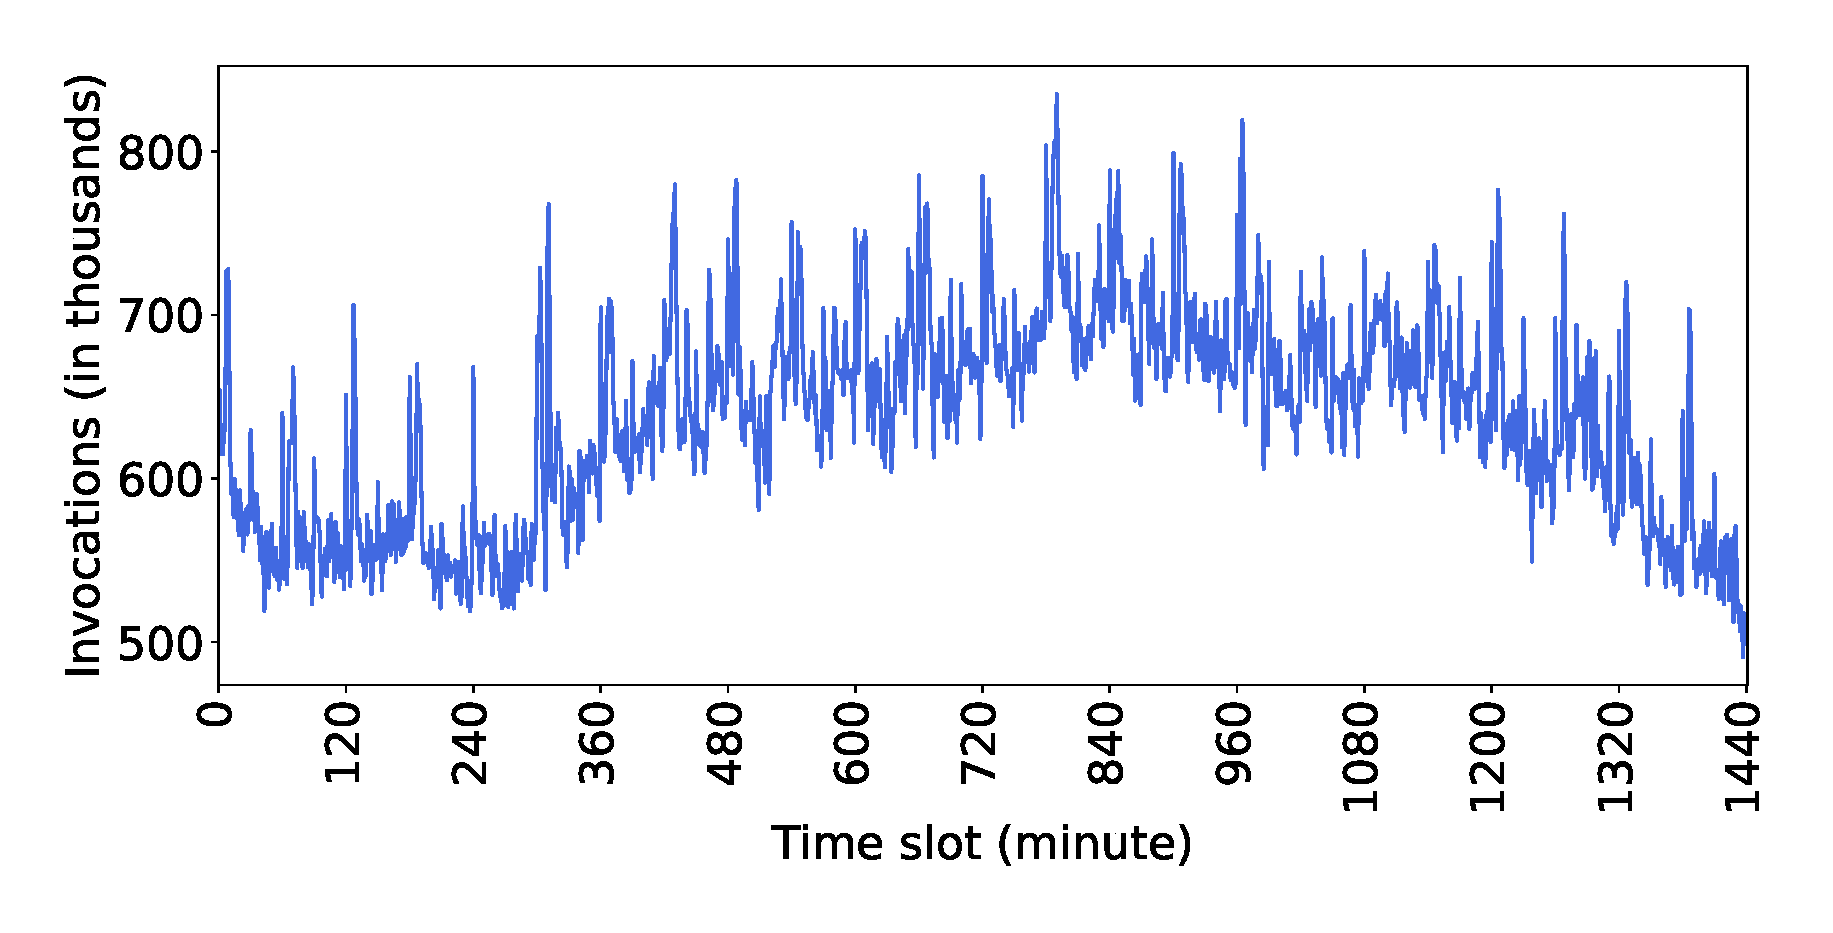
\includegraphics[width=\columnwidth]{../Figures/bursty-all_triggers.eps}
    \caption{Bursty request arrivals (invocations per minute) in day 5 of the Azure Traces.}
    \label{fig:bursty:allworkloads}
\end{figure}

This heavily skewed, bursty workload has significant implications for load balancing, since we must be able to handle highly bursty functions, as well as the long tail of infrequently invoked functions.
The fairness in handling functions is an important challenge in FaaS load balancing. 

% Furthermore, in absence of a mechanism for delaying low priority functions, serverless clusters must be provisioned for the peaks if the provider wants to be able to handle them.\footnote{Dynamically sizing clusters may be an alternative for cloud providers but not available for private clouds; but even then, allocating new VMs may be not responsive enough for sudden peaks, and high priority functions would likely suffer while the cluster is scaling up.}
% For example, we can perform a simple analysis based only on counting invocations using the data from Figure~\ref{fig:bursty:allworkloads}: Assuming a cluster that is provisioned to handle a burst up to 5\% higher than the highest observed peak in the workload, this leads to an average cluster utilization of 73\% (day 5 in Azure trace); if delaying functions is an option, a smaller cluster of 80\% of the original cluster size could handle the same workload and achieve a higher utilization (91\%).


\begin{comment}
%\vspace*{-0.2cm}
\subsection{Function Performance and Server Load}
\label{subsec:function-perf}
% Here or next section?

Our goal is to minimize the total end-to-end function execution latency. 
Unlike classic data-oriented load-balancing, function execution latency can be highly sensitive to the server load.
That is, running on an overloaded server (even if it is a warm-start), can result in significant latency increase and performance degradation.

Function performance can be affected by many factors such as the number of concurrently running functions, the CPU utilization, the load-average, interference due to other co-located functions, etc.
The slowdown in a processor-sharing system due to system load has been well modeled.
Queueing theory approaches for G/G/PS systems approximate the running time of a task to be proportional to $1/1-\rho$, where $\rho$ is the system utilization/load.

However, function heterogeneity and their execution characteristics presents many challenges in modeling and understanding their performance.
We have found that the container initialization and other OpenWhisk overheads, \emph{even for warm starts}, can be a significant source of latency, slowdown, and jitter. 

% \begin{table}
%   \begin{tabular}{ c c c c }
% \hline
%   Application & Min Time (s) & Mean Time (s) & $99^{th}$ Pctl (s) \\ 
% \hline
%   Web-serving & 0.015 & 0.408 & 1.049 \\  
%   ML Inference (CNN) & 0.166 & 0.405 & 2.299 \\
%   Disk-bench (dd) & 0.016 & 1.123 & 2.534 \\  
%   % float & 0.014 & 0.148 & 1.026 \\  
%   % gzip & 0.014 & 0.157 & 1.065 \\  
%   % image & 0.014 & 0.213 & 2.697 \\  
%   Matrix Multiply & 0.013 & 0.159 & 1.054 \\  
%   Sklearn Regression & 0.15 & 2.32 & 11.06 \\  
%   AES Encryption & 0.015 & 0.171 & 1.221 \\  
%   Video Encoding & 0.15 & 1.138 & 9.96 \\  
%   JSON Parsing & 0.015 & 0.159 & 1.012 \\
% \hline
% \end{tabular}
% \caption{The system overhead on warm invocations for the functions from Table~\ref{tab:func-times} are surprisingly high, up to several seconds in the worst case. Times were taken under load from our experiments described in Section~\ref{sec:policy-comare}. }
% \label{tab:overhead-times}
% \end{table}


\noindent \textbf{Function Jitter.}
To understand how system conditions can affect runtime of our functions, we first track their end-to-end latencies while the system is empty. 
In Figure~\ref{fig:UnstableEmpty}, we run each function repeatedly until we have 15 warm runs, then normalize those warm times by the minimum run and plot the results as a violin.
Surprisingly most functions have wildly inconsistent runtimes, ranging from 2x to 20x!
OpenWhisk traverses a complicated code path with several network hops in order to run user code, even on a warm start. 
% We describe the path briefly here to demonstrate where the varied latencies are coming from:
% \begin{enumerate}
%   \item An invocation enters system and is routed to a server
%   \item A container is chosen and arguments are sent to it
%   \item The results are stored in an external in-memory database
%   \item The load balancer is informed of completion
%   \item It must retrieve the results from the database
%   \item Results are finally returned to the user
% \end{enumerate}
We recorded the minimum time for all this OpenWhisk overhead to be $0.015$ seconds, the \emph{average} was a shockingly high 0.5 seconds, and the $99^{th}$ percentile reached 5 seconds. 
These high system overheads are largely caused by write-contention on the shared databases OpenWhisk maintains for tracking functions and their results. 
% The few that are stable are long-running and CPU bound, performing video and image transcription or ML workloads.
This high-variance system overhead  most strongly affects short running functions, but negatively affects everything in the system.
Such significant jitter motivates our stale-load aware load balancing policy, which we develop in the next section. 

% 1) load balancing bit, send to invoker
% 2) find container in pool
% 3) send args to container
% 4) put result in CouchDb
% 5) Inform controller/LB that func is done
% 6) retrieve result from LB
% 7) return to user

% Min:0.015, Avg: 0.5s, p99: 5s 

\begin{figure}
  \includegraphics[width=0.33\textwidth]{../figs/ow/function_breakdown_min.pdf}
 % \vspace*{-0.25cm}
  \caption{Functions' warm latencies vary widely even under no system load, due to OpenWhisk jitter.}
  \label{fig:UnstableEmpty}
 %   \vspace*{-0.25cm}
  %XXX:Y Axis: Normalized latency
\end{figure}


% We also place the system under some load and examine how much of the end-to-end latency is spent in non-function computation.
% All functions, listed in Table~\ref{tab:overhead-times}, have a similar minimum overhead time of over one-hundreth of a second.
% While this is a significant time, the median times are all an order of magnitude higher.
% Fully half of function invocaitons spend a tenth of a second -often much more- stuck in the OpenWhisk pipeline.
% The baseline overhead time comes from the composite services of OpenWhisk communicating to invoke each function.
% Some of the more severe times we examined had the invoker waiting several seconds trying to inform the controller of a completed execution.
% The significant jitter encourages the use of a stale-load aware load balancing policy that is agnostic to such jitter.
% These forms of jitter mean that we cannot have an ``optimal'' load balancing policy from a latency perspective, as too many external variable affect a function's end-to-end latency.


\noindent \textbf{Load-sensitivity.} 
Furthermore, we have found that \emph{different functions are affected by server load differently.}
%
Figure~\ref{fig:LatencyVsLoad} shows the correlation between function latency and the Linux load-average of the server for different function types. 
The load-average is normalized to the number of CPU cores: thus a load-average of 2 in the figure for the 16-CPU VMs corresponds to a Linux load-average of 32.
The load on the servers was increased by increasing the number of concurrently executing functions of the same type.


We see that in general, as the server load increases, so does the latency of the function invocations.
Each point in the scatter-plots of Figure~\ref{fig:LatencyVsLoad} represents a unique invocation, with the latencies normalized to the lowest execution latency observed for that function.

The AES encryption function (Figure~\ref{fig:AES}) shows a gradual increase in latency as the load increases.
Surprisingly, the effect of load is minimal: the latency increases by ``only'' 2x even at a 10x load. 
%Nevertheless, does get affected by load, but surprisingly only under extreme cases where load is over 5!
The longer-running ML training function (Figure~\ref{fig:TRAIN}) also sees a correlation between server load and its end-to-end latency.
However, it's latency variance is lower because the longer running time (50 seconds) hides the variable OpenWhisk overhead.
Both functions presented here have the highest correlation between system load and latency, yet themselves do not have a high correlation.
Thus scheduling on an overloaded server can degrade function performance, it must be weighed against the performance penalty of a cold start.
% We describe this OpenWhisk ``system overhead'' more in Section~\ref{sec:unstable-latency}.
% Thus, running warm functions on overloaded functions comes with performance degradation risk, which is highly variable and hard to model, which presents yet another load-balancing challenge. 

%Note that while it's worst-case latency was 1.6 times the ideal, that represents an additional \emph{30 seconds} until it completes.
% \textbf{Alex: Earlier text said TRAIN had high correlation. But it doesnt (axes are not the same). It only shows less variance.}
%Certain functions see essentially no impact from server load, such as the web-server in Figure~\ref{fig:CHAM}, because they do not use much CPU or have extended runtimes.


\begin{figure}
  %\subfloat[]{\includegraphics[width=0.22\textwidth]{../figs/lat-under-load/filtered/latency_to_load-loadAvg-cham.png} \label{fig:CHAM}}
  \subfloat{\includegraphics[width=0.22\textwidth]{../figs/lat-under-load/filtered/latency_to_load-loadAvg-aes.png} \label{fig:AES}}
  \subfloat{\includegraphics[width=0.22\textwidth]{../figs/lat-under-load/filtered/latency_to_load-loadAvg-train.png} \label{fig:TRAIN}}
%    \vspace*{-0.25cm}
  \caption{Latency increases due to system load, but is function-dependent.}
  \label{fig:LatencyVsLoad}
%  \vspace*{-0.25cm}
\end{figure}

\end{comment}

% CH with bounded loads is a good idea, but 
% In a large cluster, cant assume perfect load information, which is especially challenging for
% Stale loads (Dahlin) and follow-up work: homogenenous requests making it easy to predict what the server load is going to be based on the number of requests sent. But not applicable here. 




%%% Local Variables:
%%% mode: latex
%%% TeX-master: "paper"
%%% End:


% case for priorities?

\label{sec:motivation}

\section{Function Prioritization Motivation}

\begin{table*}
  \caption{Delay-tolerant scenarios. The ID of the use case is taken from a public dataset~\cite{Eismann:zenodo:2021:dataset}. We studied each case and estimate a likely delay tolerance for that scenario.}
  \label{tab:examples}
  \centering
  \begin{tabular}{lrll}
    \toprule
    Trigger group & ID & Delay     & Description \\
                  &    & tolerance & \\
    \midrule
    timer & 6 & $<$10min & NetApp's cloud function to periodically find unutilized EBS volumes to delete. \\
    event & 28 & $<$60min & Google Analytics clone to track website visitors. \\ %Note from Cristina: Google Analytics updates statistics every 24-48 hours for standard accounts 
    queue & 59 & $<$60min & Messenger Chatbot for a media company; sends weekly news updates to user. \\
    storage & 30 & $<$10min & Serverless Galleria, for batch manipulation and publishing of images. \\
    orchestration & 12 & $<$24h & Subscription fulfillment for online and print subscriptions of The Guardian. \\
    others & 101 & $<$10min & Scientific task, batch, on demand, for sequence alignment of protein sequences. \\
  \bottomrule
\end{tabular}
\end{table*}

In this section, we show that---in opposition to what others have argued in the past~\cite{Wiesner:Middleware:2021:TemporalShifting}---(some) real serverless workloads \emph{are} delay tolerant (\S~\ref{sec:motivation:delay-tolerant}), we discuss the current status of differentiated serverless functions (\S~\ref{sec:motivation:currentStatus}) and provide a workload characterization based on dividing functions into high- and low-priority classes (\S~\ref{sec:motivation:workload}).
Our study of the delay tolerance of serverless functions is based on a recent dataset of serverless applications~\cite{Eismann:Software:2021:Why,Eismann:TSE:2021:CommunityConsensus}.
For the workload characterization, we analyze traces with real serverless workloads from Microsoft Azure~\cite{Shahrad:ATC:2020:ServerlessInTheWild} and present the results of one representative day (day 5 of the 2-week trace).
%we have released the code used for the analysis in this section.\footnote{GiHub link blinded for review.}

\subsection{Can Serverless Functions be Delayed?}
\label{sec:motivation:delay-tolerant}
In this subsection, we analyze if serverless functions can tolerate some level of delay in their execution. 
This delay could come from not executing the function immediately (e.g. through queueing), or via reduced priority in scheduling (e.g. giving less resources to lower-priority functions).
While these two mechanisms differ, the result of both is increasing the turnaround time of the functions; this increase is not appropriate for some functions---like those supporting interactive or real-time applications---but is tolerable for multiple other applications, as discussed in this subsection.

Serverless functions can be triggered through several mechanisms like http invocations, cloud-native events, queue messages and timers.
Functions triggered by http are time sensitive as these are synchronous requests that can timeout and are often used in interactive applications;
all other triggers invoke functions that can tolerate delays to varying degrees.
Thus, functions not triggered by http are (potentially) delayable; in the Azure trace, these constitute $59.06\%$ of the functions and $69.07\%$ of the invocations.

Furthermore, a recent survey of serverless use cases~\cite{Eismann:TSE:2021:CommunityConsensus} found that 66\% of applications in a large dataset have at least one delay-tolerant function.
To further illustrate our point, we analyzed the applications in the dataset and selected one delay-tolerant scenario for each of the triggers (except http, which is not delayable as already explained);
these scenarios are described in Table~\ref{tab:examples} and include examples such as removing unutilized EBS volumes, a web analytics (clickstream) application, a messenger chatbot, a batch image manipulation application for a serverless galleria, a subscription fulfillment application for The Guardian, and an application for sequence alignment of protein sequences.

A note on http-triggered functions: Some web applications need end users to invoke asynchronous behavior via http requests.
The Microsoft Azure Cloud Design Patterns documentation~\cite{Eastbury:2022:Azure:AsyncPattern} provides a solution to this problem with the ``Asynchronous Request-Reply'' pattern which disaggregates such behavior into three functions: two http-triggered ones (to enqueue request and to check status of job), and a queue-triggered backend function.
In this scenario, the http-triggered functions are not delay tolerant, but the queue-triggered function is.
%(though it may tolerate only a small delay depending on the specific use case).


\subsection{Current Status of Differentiated FaaS Invocations}
\label{sec:motivation:currentStatus}
A recent empirical study~\cite{Tariq:SOCC:2020:Sequoia} found that current cloud providers (AWS, Azure, GCP and IBM) treat http functions differently from those triggered by other means, frequently via undocumented behavior, including different concurrency limits and prioritization versus background functions.
In addition, while asynchronous functions are queued and thus the user understands that they may not execute immediately, providers don't typically enqueue synchronous functions but rather return with an error if peak exceeds concurrency limits or provider capacity.\footnote{An exception is GCP which handles synchronous calls in best effort fashion, performing queuing but not ensuring zero drops~\cite{Tariq:SOCC:2020:Sequoia}.}
%
Thus, the major public cloud providers are already implicitly defining two classes of functions: high priority (synchronous) and lower priority (asynchronous), with the latter being delay-tolerant.
%asynchronous functions in AWS can be queued up to 6 hours.\footnote{\url{https://docs.aws.amazon.com/lambda/latest/dg/invocation-async.html}}
%Asynchronous functions are either explicitly (for example, with the \texttt{async} keyword in OpenWhisk) or implicitly (by its trigger) defined in current platforms.
%The asynchronous functions are good candidates to be delayed if needed.

In OpenWhisk asynchronous functions are defined with the \texttt{async} keyword and follow a different execution path than synchronous ones.
However, the platform does not use any mechanism to delay or execute them at a lower priority.
A solution that treats \texttt{async} functions as delay-tolerant, scheduled with a lower priority than synchronous functions, can be added to OpenWhisk without API modifications.

\subsection{High- and Low-Priority Workloads}
\label{sec:motivation:workload}
%Re-write section: try to make more compact 1-2 paragraphs is better
Considering the two function classes described in the prior subsection---high and low priority---we analyze the Azure traces applying this division in the workload.
For the high priority class, we consider http-triggered functions.
For the low priority class, we consider all other functions.

%\paragraph{Prevalence in workload}
High-priority functions constitute a significant portion of the workload, though the low-priority functions are greater in number and account for more than 2/3 of the invocations.
Specifically, high-priority functions constitute $41\%$ of the functions and $31\%$ of the invocations, versus $59\%$ of the functions and $69\%$ of the invocations for the low-priority.
%Higher precision numbers:
%$40.94\%$,  $30.93\%$
%$59.06\%$, $69.07\%$ 

%\paragraph{Function duration}
Figure~\ref{fig:CDF:workload} (Left) shows the cumulative distribution function (CDF) of the average function durations.
%; the dataset does not contain the duration of each invocation, just per-function aggregate statistics.
The function durations are similar for both classes, with high-priority functions being slightly shorter (median 0.2 vs 0.8 minutes).
%\paragraph{Interarrivals}
Figure~\ref{fig:CDF:workload} (Right) shows the CDF of the per-function average inter-arrivals;
%The dataset contains arrivals aggregated at per-minute intervals, making it impossible to get low granularity statistics for interarrivals smaller than one minute; most (98.8\%) interarrivals fall in this category.
the IATs for both classes are similar.
%---at the granularity that we can do the analysis---

% \begin{figure}[t]
%     \centering
%     \includegraphics[width=0.8\columnwidth]{../Figures/CDF-functionDurationsByPriority.eps}
%     \caption{CDF of the function durations, with functions divided into two groups: high-priority and low-priority.}
%     \label{fig:CDF:durationByPriority}
% \end{figure}

\begin{figure}[t]
    \centering
    \begin{minipage}{0.49\linewidth}\vspace{0pt}%
        \includegraphics[width=\linewidth]{chrlu/qos/Figures/CDF-functionDurationsByPriority.eps}
    \end{minipage}
    \begin{minipage}{0.48\linewidth}\vspace{-5pt}%
        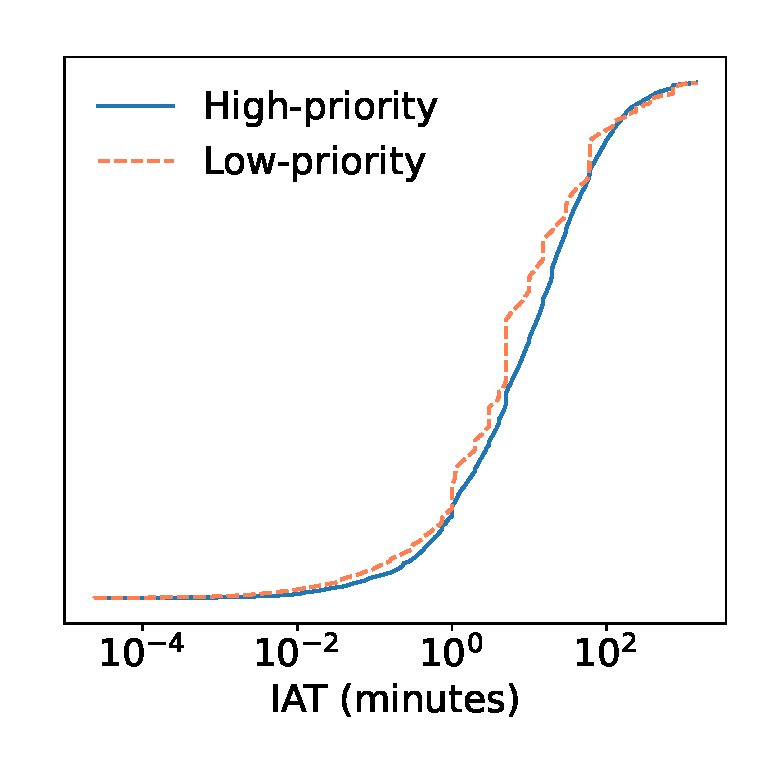
\includegraphics[width=0.95\linewidth]{chrlu/qos/Figures/CDF-averageInterarrivals.eps}
    \end{minipage}
    %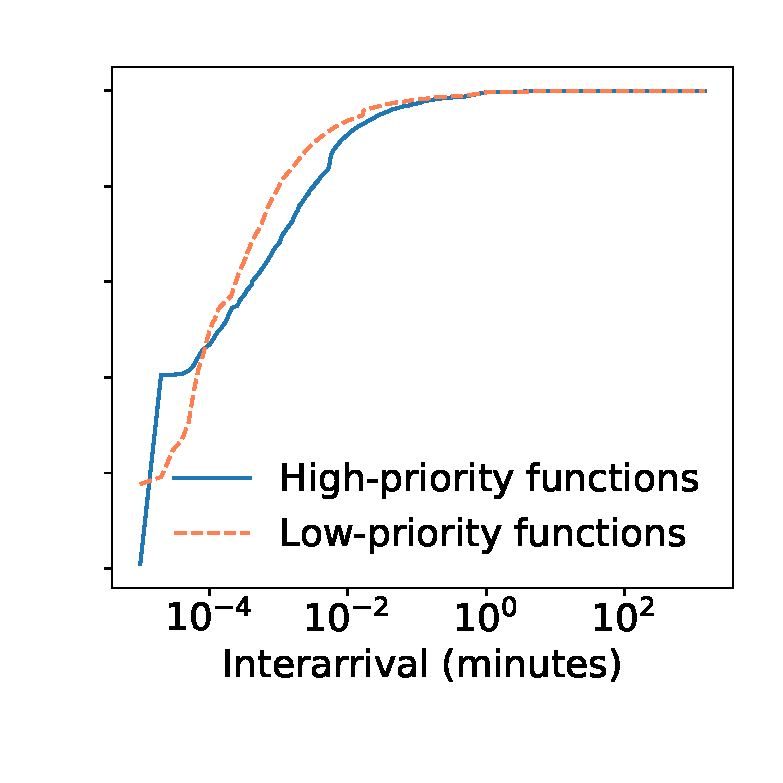
\includegraphics[width=0.49\columnwidth]{../Figures/CDF-interarrivals.eps}
    \caption{Left: CDF of the function durations. Right: CDF of the average function inter-arrivals. Functions are divided into two classes: high and low priority.}
    \label{fig:CDF:workload}
\end{figure}


% \begin{figure}[t]
%     \centering
%     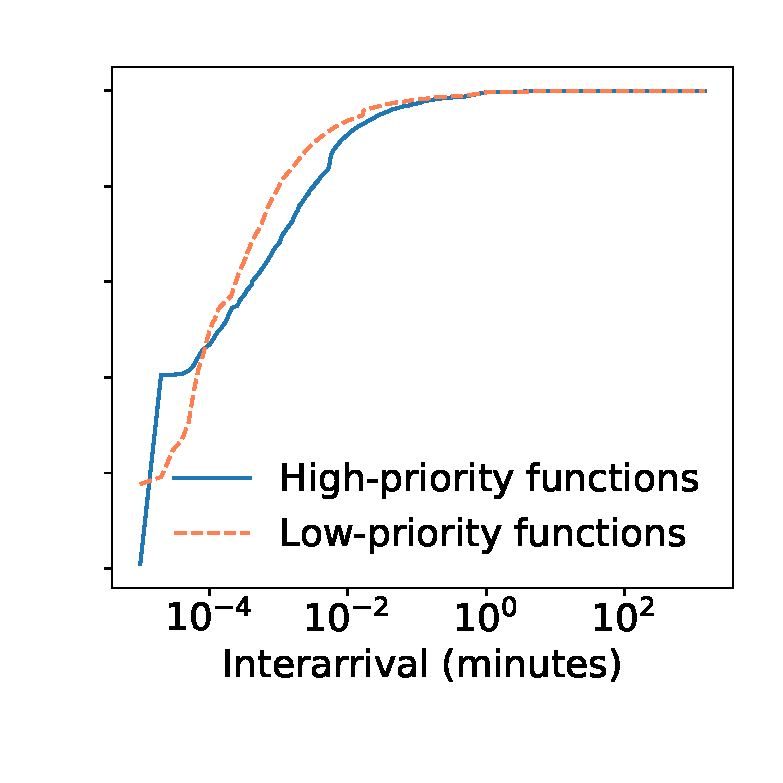
\includegraphics[width=0.8\columnwidth]{../Figures/CDF-interarrivals.eps}
%     \caption{CDF of the per-function interarrivals, with functions divided into two groups: high-priority and low-priority.}
%     \label{fig:CDF:interarrivalsByPriority}
% \end{figure}

\begin{comment}
\paragraph{Burstiness}
Figure~\ref{fig:bursty:highVsLowNormalized} shows the per-minute invocations, with functions divided into high and low priority groups and with invocations normalized to their peaks.
Both groups have similar burstiness: high-priority ($IDC=0.0083, \sigma=0.0794$) and low-priority ($IDC=0.0079, \sigma=0.0764$).
Even though the burstiness is similar, the peaks may or may not align during the 24-hour period.

\begin{figure}[t]
    \centering
    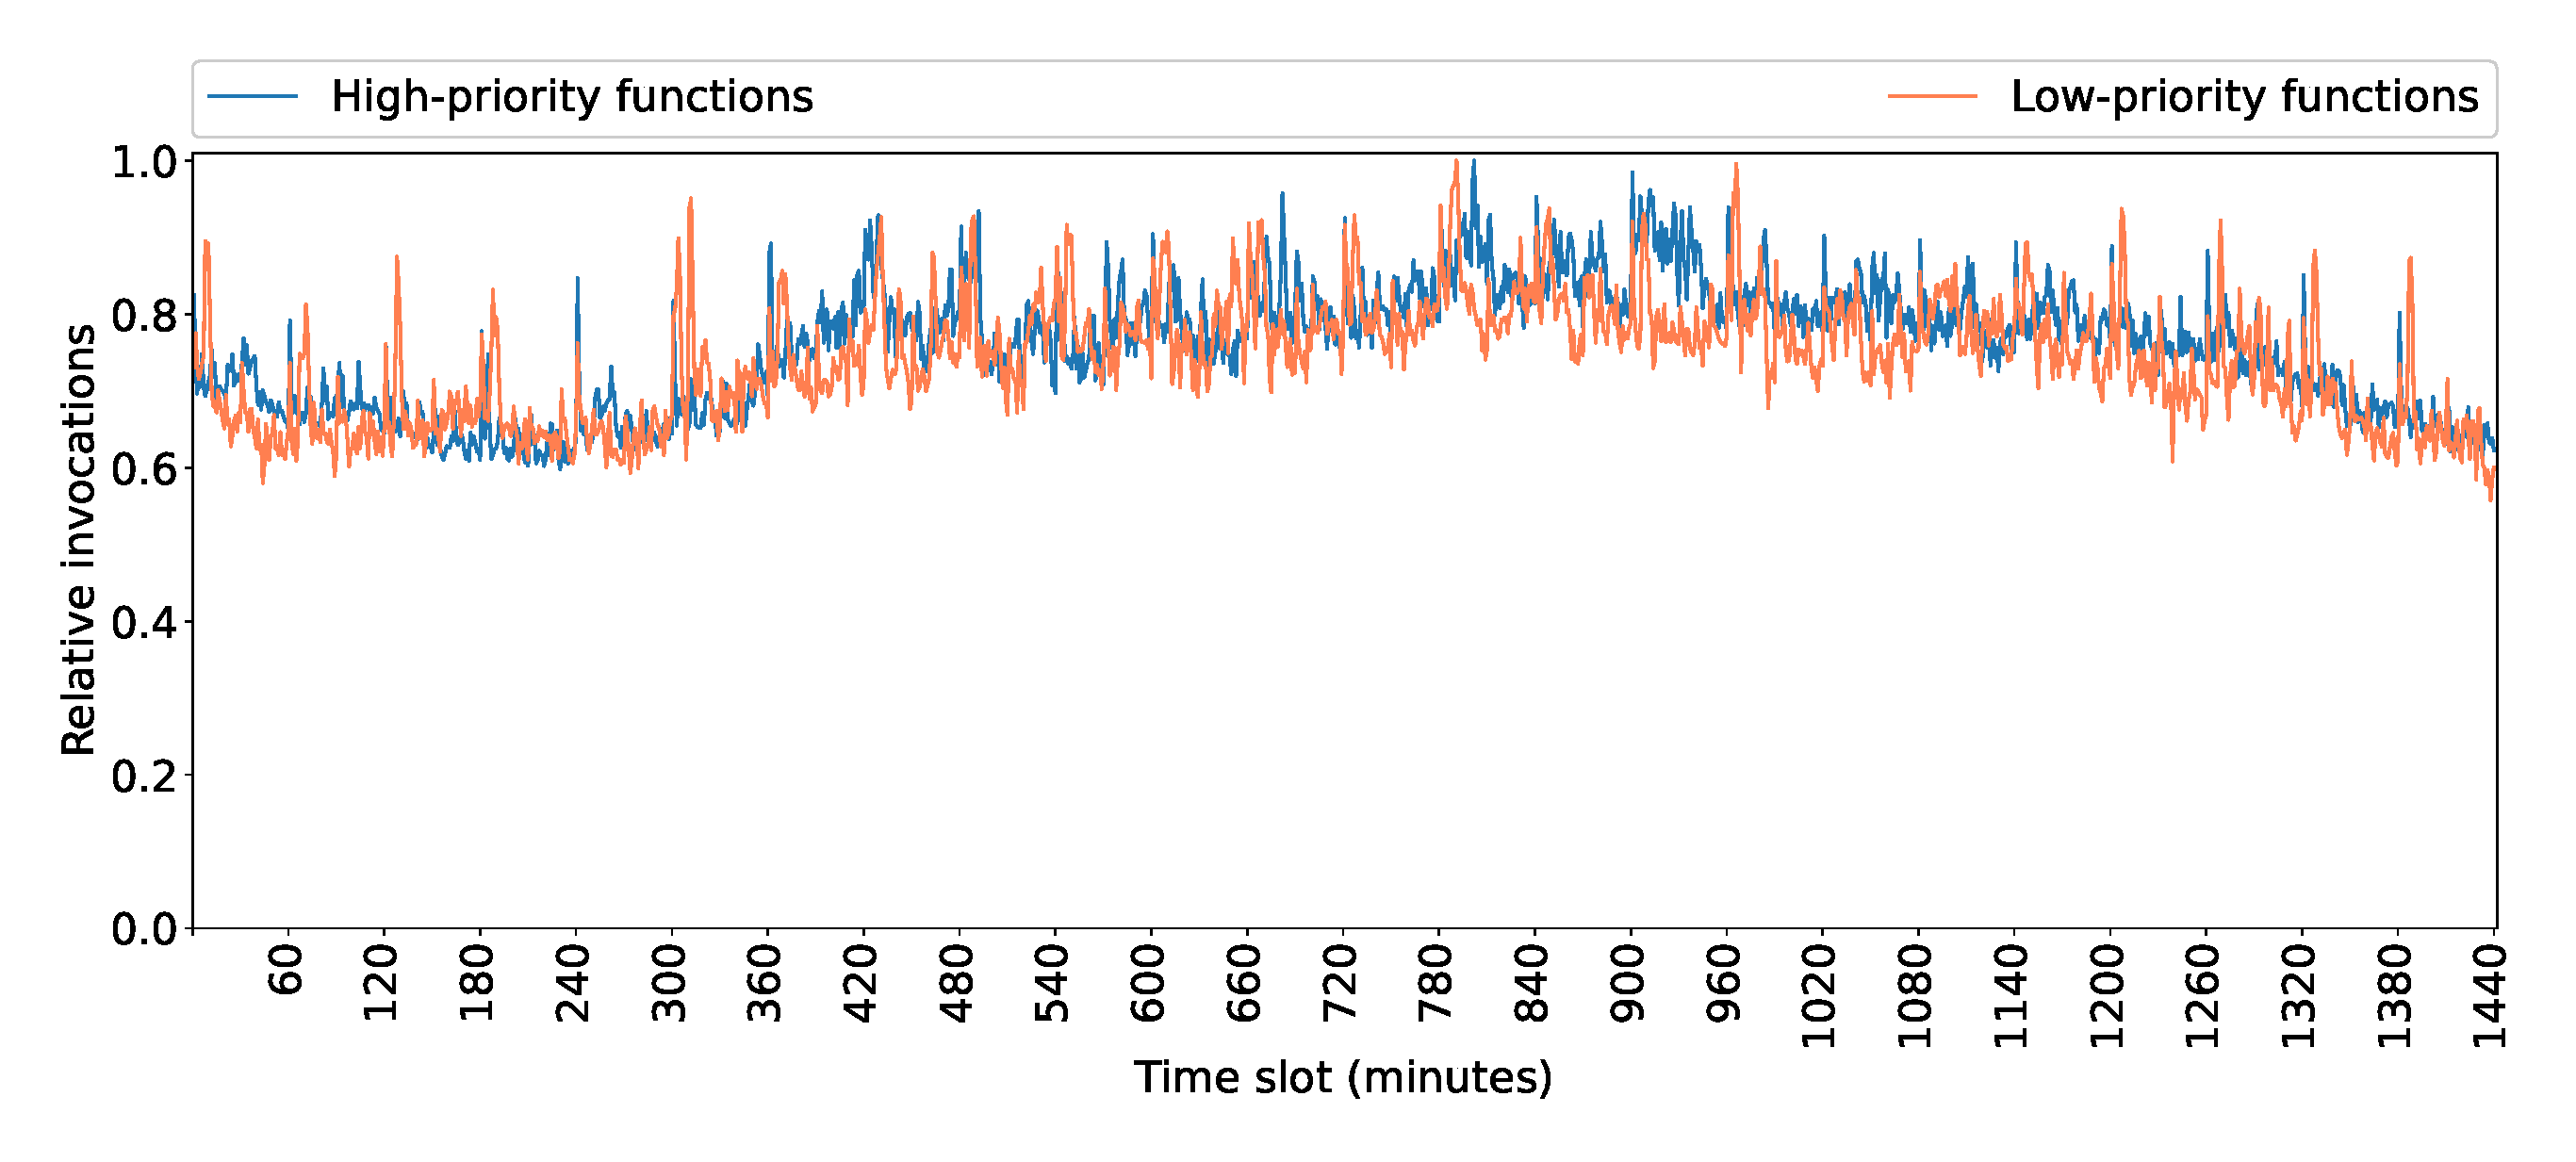
\includegraphics[width=\columnwidth]{../Figures/bursty-HighVsLowNormalized.eps}
    \caption{Invocations per minute, normalized to their peak, with functions divided into high- and low-priority groups.}
    \label{fig:bursty:highVsLowNormalized}
    % High-priority functions: 
    %   standard deviation :  0.0794
    %   IDC:  0.0083
    % Low-priority functions: 
    %   standard deviation :  0.0764
    %   IDC:  0.0079
\end{figure}
\end{comment}


%%% Local Variables:
%%% mode: latex
%%% TeX-master: "paper"
%%% End:


\section{Priority Based Consistent Hashing} % Based Load Balancing Policies}
\label{sec:qos-chrlu}

In this section, we extend the load-balancing algorithm to take into consideration function \emph{priority}, in addition to the characteristics in Section~\ref{sec:chrlu}. 
% We assume a cluster of homogeneous servers, and that a new function invocation can be sent to any of the servers.
% Each server implements keep-alive for functions: after successful execution, the function's container is stored in server memory, and evicted based on some eviction policy.

\begin{figure}
\centering
  \includegraphics[width=0.8\textwidth]{chrlu/qos/figs/k-rlu2.pdf}
  \caption{$k$-CH-RLU partitions a cluster into multiple server pools and runs server-load-aware consistent hashing in each pool. Functions are forwarded if servers are overloaded, or to a lower-priority pool if the entire pool is.}
  \label{fig:2-pool-arch}
\end{figure}

% Overview of the architecture. 
\subsection{Quality of Service Architecture}

To support quality of service (QoS) for functions of different priority levels, we use a two-stage load-balancing architecture (see Figure~\ref{fig:2-pool-arch}). 
The cluster is partitioned into multiple pools, one for each priority level.
For ease of exposition and without loss of generality, we consider two levels: high- and low-priority functions, and thus two corresponding pools. 
Within a single pool, functions are load-balanced among servers using a load-aware consistent hashing technique. 
Our approach is modular: each pool runs an independent load-balancing policy, which is the focus of most of this section. 
This approach also preserves function locality, which is important for reducing cold-starts, as we describe next.  

\subsection{$k$-CH-RLU}
\label{subsec:kchrlu}

Our overall policy, Consistent Hashing with Random Load and Updates with $k$ pools ($k$-CH-RLU), combines all the previously described techniques and insights.

Upon a new function invocation, it runs in its pool using the \texttt{forward} procedure in Algorithm~\ref{algo:PopularRLUPolicy}, which combines the use of SHARDS for popularity detection, cold and warm times for increasing the effective load bound, and noisy loads. 
The initial server is determined using a consistent hashing function. 
We bound the cold/warm ratio with a final load upper bound, $b\_max$.
The load-bound parameters determine the locality sensitivity: higher values of $b$ and $b\_max$ increase locality at the risk of resource-contention delays.
Similarly, higher values of $p$ results in more aggressive random forwarding and reduces locality. 

Our two-level architecture is modular and allows us to parameterize different load-balancing policies for different pools.
Lower-priority pools are run with a higher load bound $b\_max$, and thus tolerate more overloaded servers, at the risk of lower function performance.
Forwarding along the chain has diminishing returns on locality, and if the function gets forwarded more than $max\_chain\_len$ times, it triggers the overflow condition.

Function prioritization and QoS are controlled via the server pools: Each function has a default pool based on their priority level, with higher-priority functions having lower pool numbers. 
The high-priority functions recursively overflow to the next lower-priority pool, and thus have good locality because all pools use our consistent hashing approach. 
The high-priority functions can thus overflow and potentially use the entire cluster in case of workload spikes, preserving their QoS. 
The lower-priority pools thus also serve as a ``burst buffer'', crucial considering the bursty nature of functions. 
Low-priority functions can't make use of higher-priority servers even if they are available, since we want to be able to handle bursty invocations of higher-priority functions. 
For the lowest-priority pool, we run the function on the least-loaded server in their pool. 
%
If the least loaded server is also overloaded, we drop the function.
% \begin{figure}
% \begin{algorithm}[t]
%   \caption{$k$-CH-RLU}
%   \begin{algorithmic}[1]
%     \Procedure{forward}{$pool, func, server, chain\_len $}
%     \State $b, b\_max, max\_chain\_len \gets system\_params $
%     \If{$ chain\_len > max\_chain\_len $} \Comment Overflow 
%     \If{$ pool == k $} \Comment Lowest-priority pool
%     return least-loaded-server
%     \Else \State forward(pool+1, func, server=CH(func, pool), 0) \Comment Try in next pool 
%     \EndIf 
%     \EndIf 

%     \State $\lambda \gets 1.0 / avg\_iat$ \Comment Computed from Algo 1
%      \State $L=Load(server)$
%     \If{popular(func)} \Comment Computed from Algo 1 
%          \State $L = Load(server) + \mathcal{N}(\mu=\lambda\,\sigma=0.1)$
%     \EndIf 
%     \If{$L < min(cb/w, b\_max)$}
%        \State server
% \Else \State forward(pool, func, next(server), chain\_len+1)
%        \EndIf
%        \EndProcedure
%     \end{algorithmic}
% \label{algo:PopularRLUPolicy}
% \end{algorithm}

% \begin{algorithm}
  
% \end{algorithm}



\noindent \textbf{Pool Sizing.}
The priority pools are sized proportional to the number of functions registered at different priority levels.
Thus, if 25\% of all functions are low-priority, then 25\% of the servers are in the low-priority pool and the rest are in the high-priority pool.
Periodically, we recompute this ratio based on the currently registered functions, which may lead to resizing the pools.
Importantly, locality is preserved even after pool resizing because of consistent hashing. 


\begin{comment}
We have also implemented a simple PID controller with hysteresis for horizontal scaling, by using server load averages as the input control signal. 
This horizontal scaling is conservative, with a large dead-band of 5 minutes, and scaling is triggered only if the at least 50\% of the servers are overloaded.
As we shall show in the empirical evaluation, CH-RLU significantly reduces the variance in the loads among servers, and thus is more amenable to this horizontal scaling policy. 
\end{comment}


% Unpopular functions still use Algorithm~\ref{algo:ConsistentCachePolicy}.
% In all cases, if we exhaust the list of servers trying to find one with low load, we randomly assign the invocation to a server.
% This only occurs in the most extreme cases of system load and also prevents spamming a popular server in that same scenario.



% if popular: L+Noise > bound 
% else: L > bound 

%%% Local Variables:
%%% mode: latex
%%% TeX-master: "paper"
%%% End:


%\section{QoS Policy}

Users provide the QoS priority. Currently binary: high and low priority. 

\subsection{QoS Policy Tradeoffs and Challenges}

There are many possible paths towards realizing QoS differentiation on FaaS clusters, and we now discuss different possible approaches and their tradeoffs.

\paragraph{Cgroups.} We can enforce service differentiation at the \emph{server} level: and use the virtual environment's resource allocation and control mechanisms.
For instance, we can use cgroups to reduce the relative and absolute cpu and memory allocation of the low-priority function containers.
While this approach is feasible, it has some drawbacks.
Mainly, using cgroups only controls the resource footprint of the actual function execution.

However as we saw in the previous section, a significant, often majority, time is spent in the various function initialization steps.
This initialization is not necessarily part of the ``function context'', and thus not directly controllable through cgroups-like mechanisms.
Significant resource consumption occurs in initializing the function for cold starts and \emph{even for warm starts.}
Specifically, we found that unpausing a docker container and allocating network interfaces to it can consume significant CPU resources.

However, this resource consumption occurs as part of the FaaS ``control plane'', i.e., OpenWhisk, Docker, kernel components for networking, namespaces, and cgroups.
Using cgroups to reduce resource allocation by reducing the cgroup priority/quotas/limits only reduces function execution speed, but misses the significant (and often the majority) resource consumption in the control plane.
Thus,
\todocristina{Last paragraph is incomplete; other than that, we need a figure for the unpausing docker container experiment.}

\paragraph{Queueing at the server.}
Another server-level approach is to introduce a queue at each server, which can prioritize function execution by delaying low-priority functions.
This can be a  powerful approach in general.
Priority queueing algorithms often assume some deterministic or a probability distribution of service times of the different jobs such as exponential distributions.

However, function execution times, due to the control-plane overheads, show a very high variance, and their execution time is not exponentially distributed.
Moreover, function execution times are highly heterogenenous, and servers run 100s of different functions, which makes analytical solutions non-trivial. \todocristina{Do we know that function durations are not exponentially distributed?}

\textbf{Need to tighten this argument, or remove it.}

Server-level throttling either using cgroups or queueing also has more general tradeoffs. 
If all servers are available for a delayable function to use, then idle servers can be used to opportunistically run them. 
However, this may lead to poorer locality (i.e., more cold-starts), and increased risk of performance interference between high and low priority functions. 

% Our approach : 

\subsection{Our approach: Cluster Pools}

Key idea is to have a separate pool of servers for running the low-priority delayable functions. 
The high priority pool handles the conventional functions. 

Within each pool, we use a locality-aware load-balancing policy to reduce the effects of cold-starts and server loads. 

\subsection{Low priority pool as Burst buffer}

Low priority servers can be used to handle high priority invocations in case of bursty invocations that are quite common.

We integrate load balancing with cluster pools to handle workload bursts.

\begin{itemize}
\item Locality is important, so we must build on consistent hashing. 
\item However, consistent hashing alone results in overloaded servers because of the heavily skewed workload (1\% functions taking 90\% resources, etc.)
\item This is fixed with bounded loads and forwarding. Make sure each server has a max capacity. For a new invocation will exceed this capacity, it is forwarded along the ring. 
\item For bursty functions, even this may be suboptimal, since a sudden burst of invocations can saturate many consecutive servers, starving other functions of warm hits. 
\item Thus, recently, CH-RLU has been proposed: which adds a random load to each server for popular functions, to forward popular functions more aggressively. 
\item We build on CH-RLU. 
\item For forwarding functions, we set a max forward limit (the chain length). If we exceed the chain length, \emph{our key idea is to run the function on the low-priority cluster pool.} Currently, CH-RLU will run function on least-loaded server, breaking locality. 
\item Our key new idea also preserves locality. Popular functions likely to run on the same subset of servers in the low priority pool. 
\item Low-priority pool continues to use CH-RLU without any overflowing. 
\item Thus bursts can be quickly handled without slow and expensive repartitions. 
\item We call our policy ``CH-RLO'': Consistent Hashing with Random Loads and Overflow. 
\end{itemize}


\subsection{Partitioning Policy}

Assume we have a fixed number of servers, $S$. 
Out of these, $x$ are for the high-priority functions, and the remaining $S-x$ for the low-priority functions. 
The ultimate goal of the partitioning policy is to decide what $x$ should be. For this, we use a simple online control-based optimization approach. 

\textbf{Initial configuration.}
Since functions have to be registered as low or high priority, we set $x/S$ proportional to the ratio of number of high ($N_H$ )and low priority ($N_L$) functions.
Specifically, we introduce an overcommitment parameter $c$ that determines how small the low-priority pool is going to be.


\begin{equation} x_0 = c \frac{N_H}{N_L} S \end{equation}

\textbf{Adjusting x.}
Note that the invocation frequency and running time of functions can vary widely, so this initial assignment need not be ideal.
Our goal is to improve the performance of both the high and low priority functions, but deprioritize the performance of low-priority functions by a factor of $c$.
Thus, the objective function, $F$, is:
\begin{equation}
  F(x) = f_H - \frac{f_L}{c},
\end{equation}
where $f_H$ is some aggregate performance measure of all high-priority functions, and $f_L$ is for low-priority.

We use
\begin{equation}
f_H=\sum_i^{N_H} \frac{\bar{\tau_i}}{\min{\tau_i}},  
\end{equation}

where $\bar{\tau_i}$ is the average latency of function $i$. (Better symbol? L already used for Low priority). 
More concretely, the performance measure is the increase in latency. Since FaaS providers do not have access to the ``ideal'' or baseline latency, and because it can vary widely based on the function (from few ms to few minutes), it needs to be normalized. We normalize each function's latency by the minimum latency of that function observed so far. 

Our goal is to balance the cluster so that $F(x)=0$.

Thus, periodically, we use a gradient-based method: $\delta(x) = \eta F(x)$, where $\eta$ is the step size.

We can consider other objective functions too.
One appealing one is to measure the delay of functions explicitly, where delay is defined as the total latency minus the actual function execution duration. This captures the FaaS control-plane (i.e., OpenWhisk, docker and other components) overheads.



%%% Local Variables:
%%% mode: latex
%%% TeX-master: "paper"
%%% End:


%\vspace*{-0.2cm}
\section{Implementation}
\label{sec:impl}

We have implemented our consistent hashing with random load update (RLU) policy and other load-balancing policies in OpenWhisk, a popular FaaS system.
Our changes amount to more than 1,700 lines of code across many OpenWhisk components, but are primarily in the load-balancer class. 
In this section, we describe major implementation details, as well as key performance optimizations which significantly improve OpenWhisk performance and scalability by more than $4\times$. 

Our policies are implemented by modifying the load-balancer module of OpenWhisk (see Figure~\ref{fig:sys-diag}).
CH-RLU is implemented by modifying the existing OpenWhisk ``container sharding'' policy, which also uses consistent hashing, and forwards functions using only available memory as the load metric.
We use OpenWhisk's existing consistent hashing implementation, permiting an ``apples to apples'' comparison, and also making CH-RLU a ``drop-in'' replacement for the OpenWhisk default load-balancing. 
At the invoker level, we adapt FaasCache's GreedyDual keep-alive policy, which increases the keep-alive effectiveness compared to OpenWhisk's default non-resource-conserving TTL eviction~\cite{faascache-asplos21}. 

\begin{figure}  
  \centering
  \includegraphics[width=0.6\textwidth]{chrlu/faaslb-osdi22/figs/sys-diag.pdf}
 %   \vspace*{-0.3cm}
  \caption{System diagram of relevant OpenWhisk components and communication used to schedule and run function invocations.}
  \label{fig:sys-diag}
  %  \vspace*{-0.3cm}
\end{figure}

The CH-RLU algorithm described in the previous section requires two main additional pieces of information from each invoker/server: the load averages, and the cold/warm running times of functions. 
Both of these are periodically (every 5 seconds) captured and stored in a centralized redis key-value store.
The load-balancer in the controller reads these asynchronously: working with stale and inconsistent metrics is our key design goal. 
The default load-bound, b, is 1.2, and the max load, b\_max is 6. Popularity threshold is set to 20\%.
We did not observe performance to be very sensitive to these parameters, and thus do not need to auto-tune them, and they are suitable as user-inputs. 

%\vspace*{-0.2cm}
\subsection{Performance Optimizations For OpenWhisk}

Since our goal is to run functions under high load, we ran into a large number of OpenWhisk performance and scalability bottlenecks.
We found default OpenWhisk to be almost unusably slow and unstable even under reasonable load. 
We present their details and our actions to overcome them, hoping that the fast-growing serverless computing research field can benefit from our lessons. 


In our experience, the primary source of scalability bottlenecks is running Docker containers concurrently.
We found significant contention in \texttt{dockerd}, Docker's control daemon which handles all the container lifecycle events.
Even at moderate loads (normalized server load average close to 1), high dockerd contention can increase tail latencies by \emph{several minutes!}


Currently, OpenWhisk \textbf{pauses} each container after function execution, which prevents it from being scheduled by the CPU.
It then resumes the container before running the next invocation of the same function (assuming a warm start).
Thus each invocation requires these two additional (pause/resume) events to be handled by dockerd, which results in significant lock contention.
Because of the FaaS programming model, the pausing is not necessary, since nothing in the container can run after a function has returned.
Therefore, we remove these redundant pause/resume operations to reduce dockerd contention.
This reduces the OpenWhisk overhead by 0.2 seconds \emph{per-invocation} on average.
More importantly, by reducing dockerd contention, we were able to run a much larger number of concurrent functions. 

An even larger source of scalability bottleneck is \textbf{network} namespace creation time.
Using the default bridge networking requires each invocation to create a new TUN/TAP network interface.
We found this to be a very expensive operation because of Linux network stack overheads (several 100 ms), and because of dockerd's userspace lock (futex) contention for its networking database. 
We found that as the \emph{historical} total number of containers launched grows, so does the size of the network-interface database.
Dockerd reads and updates this database under the critical section, and the larger database results in higher lock contention.
As a result, we were unable to use VMs/servers with more than 4 CPUs after 20 minutes of sustained load, since the dockerd contention resulted in many functions timing out (timeout was 5 minutes)! 

We sidestep this problem by not using bridge networking, but instead using Docker's \textit{host} network option and assigning each container a unique port on the host. 
Implementing the network change required updating the OpenWhisk runtimes used to wrap functions to monitor their specified port.
This change allowed us to run functions on larger invokers and under more sustained load, and eliminated most timeouts. 

Finally, after a certain request rate threshold, we found the default \texttt{nginx} OpenWhisk frontend would crash and return \textit{502 BAD GATEWAY} for all URLs. 
We did not discover the cause of this problem, and simply bypassed it by letting function invocations to communicate with the controller/load-balancer directly. 

\noindent \textbf{CPU limits.} 
OpenWhisk uses the \textit{-{}-cpu-shares} option to set container CPU priority.
This has an unintended consequence of allowing functions to use more than one CPU core while running.
Major FaaS providers constrain functions to a single core unless they have extremely high memory allocations (<1 GB).
In order to stay in line with providers and prevent outsized impact on system load from some functions, we use the \textit{-{}-cpus} flag instead to assign each function no more than one CPU.

Together, these performance optimizations have allowed us to run OpenWhisk on invokers that are $4\times$ larger, and serve more than $6\times$ the load, without dropping functions due to timeouts.
%
We plan to upstream all these performance optimizations in OpenWhisk to provide a higher-performance and lower-jitter control plane for FaaS research and production deployments. 

\begin{comment}
\noindent \textbf{docker pause.} 
OpenWhisk pauses Docker containers after each invocation completes to prevent the user code from continuing to run.
We disable this pausing because it causes significant contention inside Docker, affecting both latency and the ability to run more concurrent functions on an individual server.
Because we control the code running inside all our functions, we do not need the pausing as a security concern or to limit impact on load.
Our functions do not do anything outside of an invocation.

\noindent \textbf{configuration.}
While OpenWhisk provides a large number of configurable settings, most of them are locked into files.
In order to make the settings more amenable to prototyping and rapid changes, we converted many of them to also work as injectable environment variables.


\end{comment}



% SPACE: can be safely removed to get space back
% OPTIMIZATION
%Finding the consistent hash node a function hashes to is a relatively expensive operation, so we simply cache these pairs for fast lookup.
% Any time we change the hash ring (i.e. an invoker comes or goes) we simply empty the cache and allow it to refill as requests come along.


% SPACE: can be safely removed to get space back

% \begin{enumerate}
%   \item docker contention
%   \item host network
%   \item OW usage of docker CPU limits
%   \item general significant OW overhead
%   \item skip nginx
%   \item make many settings configurable
% \end{enumerate}

% OW Overhead median = 0.05472302436828605 seconds
% ShardingContainerPoolBalancer [0.0215673  0.05472302 0.86742063 4.59444914 6.49693995]
% quantiles: [0.1, 0.5, 0.8, 0.90, 0.99]


\section{Experimental Evaluation}
\label{sec:eval}

% Run on system with Ubuntu, 48 phys cores, Nvidia P100 GPU, 250 Gb ram
% Here we will showcase the effectiveness of our GPU memory manipulation in minimizing
Here, we showcase the many parts of our design in an extensive series of experiments that fully analyze its impact.
All experiments were run on identical systems running Ubuntu 20.04 on kernel version 5.4, with a 48 physical core Intel Xeon Platinum 8160 with hyperthreading disabled, 250 GB of RAM, and an Nvidia P100 GPU running driver version 470.239.06.
This isn't the latest GPU hardware, and emphasizes that our design can work with a variety of hardware, doesn't require advanced features, and is easily scalable and adaptable to other systems.

\subsection{UVM Shim}
\label{sec:shim}

The piece underpinning our entire design is our driver shim that captures and rewrites memory allocations made by function code.
If we cannot oversubscribe memory or can only do so by significantly increasing code execution time, our system design is untenable.

\mhead{Memory Management}
Our shim enables two abilities, GPU memory overcommitment and control plane management of memory placement.
To show the impact of both we run 16 copies of the FFT function from Table~\ref{tab:fun-list}, each using 1.5 GB of device memory that, in aggregate, oversubscribes our GPU's memory by 50\%.
% To show the importance of locality of function memory and available space, we run 16 copies of the FFT function from Table~\ref{tab:fun-list}, each using 1.5 GB of device memory that, in aggregate, oversubscribe GPU memory by 50\%.
We then invoke them individually and iteratively 20 times such that all will be executed before starting executing the first again.
Before and after invocations, we direct our shim to prepare function memory in various ways.
The impact of these different memory policies are displayed in Figure~\ref{fig:mem-prefetch}, with average time spent in-shim shown in red and function code execution in black.
With such high oversubscription, UVM driver alone controlling data placement, the \texttt{None} case, execution time is 40\% worse than the optimal seen in Table~\ref{tab:gpu-cpu}.
Execution time is higher when memory must be paged in on-demand from the host as kernels access it, and old memory paged out.
% An intial proactive mechanism of telling the driver our data location preference, \texttt{Madvise}, tells the CUDA memory system we would prefer the memory onto the card, and after execution to prefer it off.
Using just the driver madvise mechanisms, \texttt{Madvise}, tells the CUDA memory system we would prefer memory on the card, and after execution to prefer it off.
This actually is worse than \texttt{None}, as madvise calls to the driver don't actually move any memory, we just waste time sending the memory directives with no benefit to execution time.
Active prefetching with \texttt{Prefetch To} asynchronously copies memory to the device before invocation, and \texttt{Prefetch} additionally moves data off device after execution.
If we only tell the driver to move memory \textit{onto} the device, it must spend time page swapping to fulfill our request, and potentially move pages we still need.
Combining removal of idle memory \emph{and} prefetching memory in anticipation of use reduces function latency by 33\% over \texttt{None}.
We send prefetching directives off the critical execution path, thereby reducing the latency to just execution time, which now matches the ideal execution time as listed in Table~\ref{tab:gpu-cpu}.

\begin{figure}
  \centering
  \includegraphics{mqfq/graphs/mem-move/f16-i20-driver-mps-move.pdf}
  \caption{More intelligent memory management improves execution latency. 
    \texttt{Prefetch To} moves memory on-device before a function container executes.
    \texttt{Prefetch} additionally moves it off again when the container will be idle.}
    \label{fig:mem-prefetch}
% Fetch Strat, Exec Time, Fetch Time, Total Time
% Madvise 1.4893044978380203 0.021360369771718932 1.5106648676097392
% None 1.4704825393855572 1.2621283531188965e-06 1.4704838015139103
% Prefetch To 0.830518102645874 0.4062889523804188 1.2368070550262928
% Prefetch 0.7852441824972629 0.22023404985666276 1.0054782323539257
\end{figure}


\mhead{Interception Overhead}
We intercept driver calls and replacing physical memory allocations with UVM to enable memory management, but this change comes with a price.
To determine the impact, we run each function 10 times, with and without our driver shim enabled, tracking their latency.
We never adjust where the function's memory is, so any overhead will be caused by interceptions and usage of UVM allocations.
Figure~\ref{fig:shim-overhead} collates a variety of different function types and how they were affected.
Most functions see zero added execution time from the shift to UVM, our interception being undetectable.
The rest see single-digit percentage increases, with \funcname{Srad} standing out with a 30\% overhead in execution time under the shim.
These results are in line with Nvidia's own reporting on the performance change when migrating applications to UVM~\cite{nvidia-uvm}.
With our driver having such little impact, it is ideal for enabling a warm container pool of GPU containers and moving function memory off device when idle.

\begin{figure}
  \centering
  \includegraphics{mqfq/graphs/driver-compare/8-exec_time.pdf}
  \caption{Functions see little to no impact from our interception and substitution of allocation calls.
          This matches performance promised by Nvidia for UVM applications.}
    \label{fig:shim-overhead}
\end{figure}

\subsection{Queuing Knobs}
\label{sec:queue-knobs}

Knowing we can efficiently manipulate GPU memory, we move to testing our queuing policies built on top of them.
Our queue design allows for a number of hyperparameters that are either fixed by configuration or dynamic at runtime.
Here we explore the effects of each knob in isolation to see their effect on performance.

Each experiment is run with the same trace composed of 18 functions, run for 10 minutes, have roughly 2 invocations per second, and presented results are the average of 5  repeated runs.
Function were randomly chosen from Azure trace in the same manner as previous works~\cite{fuerst2023iluvatar,faaslb-hpdc22}, and the trace generated by randomly sampling from an eCDF computed from the Azure data.
To map a function name to actual GPU code, we select the closest matching execution duration from Table~\ref{tab:gpu-cpu} that doesn't exceed that time.

\mhead{Container Pool}
% Functions running warm is vital for low latency in serverless systems which, and our UVM shim enables maintaining a warm pool of GPU containers.
To show the effectiveness of both \QName's sticky dispatching and having a container warm pool are at decreasing cold hits, we increase the number of functions to 65 while keeping the invocations per second similar.
Experiment duration is increased to one hour to prevent first-time invocations of functions, which will always be cold starts, from dominating the results.
% To show how cold hits decrease as the warm pool is enabled we increase the number of functions to 65 and the duration to one hour while keeping the invocations per second similar.
% The high number of functions will stress the need for having available containers 
The high number of functions stresses the need for having a warm pool, as is clear from the results in Figure~\ref{fig:container-pool-cold-hits}.
A simple FCFS queuing policy that has no warm pool (e.g. pool size of 1) sees colossal 90\% cold hit rate.
%  caused by both the lack of warm pool and inability to reorder enqueued invocations so that they may run warm.
% Looking at the blue line, with no pool, (e.g. a pool size of 1), 10\% of invocations run cold, which cause a knock-on effect of higher latencies for both the invocation run cold and those waiting in queue.
Comparatively with the same lack of pool, \QName~without concurrency, represented by the blue line, only has 10\% of invocations run cold.
%  kept low entirely by its locality measures.
\QName's improvement comes from its locality and overrun techniques, as FCFS cannot reorder invocations and must frequently evict container to run the next item.
% Note that \QName~doesn't intentionally optimize for running a function in a warm container, but this emerges due to its overrun and throttling policies.
% This number are low to start thanks to the locality measures in \QName, comparatively, a FCFS Naïve queuing policy sees a much higher 90\% cold hit rate.
When the pool is increased to 32 containers, only 2\% of \QName~invocations are cold, which continue to decline with higher sizes.
FCFS also benefits from the warm pool, with both policies having equal cold hits when the pool size is maximized.

When we increase concurrency (\D), two scenarios come up: either different functions run concurrently with each other, or a function runs concurrently with itself.
The latter causes higher cold starts as we need one container per dispatched invocation of the same function.
Green and orange lines in Figure~\ref{fig:container-pool-cold-hits} show the impact of \D~on cold starts.
% High numbers equivalent to the no-pool case appear, and are again mitigated by the larger pool size.
Cold hits are higher with concurrency as expected, but are mitigated once the warm pool size grows to 32.

\begin{figure}
  \centering
  \includegraphics{mqfq/graphs/container_pool/big-60min/65/cold_hits.pdf}
  \caption{\QName~greatly reduces cold hits compared to FCFS, and is improved with a large container pool size. 
          More cold hits are also caused when \D~(concurrency) is raised, needing private containers to serve concurrent invocations.}
    \label{fig:container-pool-cold-hits}
\end{figure}

\mhead{Unfairness}
The limited resources on GPUs encourages us to prefer running a function several times because its resources are already on-device.
Adjusting the maximum overrun \T~to find the ideal balance point between fairness and stickiness is important.
% Figure~\ref{fig:unfairness-queue} shows how performance can be improved by allowing some unfairness by adjusting \T, the maximum allowed overrun of a flow.
% Figure~\ref{fig:unfairness-queue} are the average of time spent in the queue, with each function's queue time being normalized by their fraction of invocations in the trace.
Figure~\ref{fig:unfairness-queue} compares the average invocation latency as we increase \T.
Using a fixed increment to \VT~(i.e. 1.0 in Figure~\ref{fig:unfairness-queue}) is a simple solution and forces functions' to have an equal \emph{number} of invocations.
Such a policy ignores functions' variable execution times, favoring those with long execution times, and as seen in many other scheduling domains leads to unfairness and poor performance.
When $\T \le 1$, each flow is immediately throttled after a completed dispatch, forcing it to lose on-device locality, and has a terrible impact on latency.
% Larger \T, up to 10, improve latency by up to 25\%, a notable benefit provided by locality,
As \T~increases, latency is improved by up to 25\% at $\T == 10$, locality causing invocations to complete faster and increasing flows drainage.

The service average by which we increase a flow's \VT~has a significant impact queuing.
Using function execution time (Wall Time) as the service average changes \VT~to represent \emph{time} on device per-function.
Execution time is highly variable in FaaS unlike MQFQ's disk I/O domain, and ignoring it can lead to unfairness.
% Small yet popular functions are frequent in FaaS, favoring them shows when the best performance.
With $\T \approx 5$, latency is 70\% better than with immediate throttling, and 60\% better at this point over the fixed service average.
When \T~becomes too large, device time is hogged by specific flows, unfairness becomes extreme, and we see worse invocation latency.
% Favoring short functions will be allowed to run several times before being replaced with a long one.
% A flow with a long-running function 

\begin{figure}
  \centering
  \includegraphics{mqfq/graphs/unfairness/25.7/e2e_sec.pdf}
  \caption{Adjusting \T~allows flows to overrun one another, increasing data locality and therefore performance.
  The performance changes when a function's GPU wall time is used to change \VT, or the increment is fixed.}
    \label{fig:unfairness-queue}
\end{figure}

\mhead{Active Flow TTL}
A larger \T~is not the only way tool design has to favor locality, we can also keep a flow \emph{active} even while empty.
Empty flows remain active until a TTL expires, then they're made inactive and have resources moved off device.
Figure~\ref{fig:flow-ttl} shows the improvement to both execution time as compared to ideal warm performance (improved by local resources), and latency (additionally improved by priority dispatching) as the TTL grows.
Setting any global TTL (the solid line), at even a small 0.1 seconds, improves latency and overhead by 25\% and 50\% respectively.
% Latency sees a 25\% improvement and execution time over 50\%, from \emph{any} TTL policy, and 
Increasing the TTL to up to 4 seconds sees significant, but diminishing, returns.

% A large 4 second time can reduce latency by 35\% and execution time by 40\%.
We can also base the TTL on each function's inter-arrival-time (IAT), rather than have a global fixed time.
This method sets the TTL for each flow to the IAT multiplied by the value on the X axis, plotted as the dashed line.
Switching generally performs better, and performs best when $TTL = IAT \times 1.5$, reducing invocation latency by 40\% over no-TTL.
These results fit the heterogeneous and bursty nature of FaaS functions with varied IATs.
Even popular functions with low IAT can have idle periods, and keeping their resources warm for short periods allows fast handling when they re-appear.
Setting the TTL too high at $IAT \times 3$ prevents them from transitioning to inactive, leaving their \VT~artificially low, jumping them unfairly ahead in the queue.

\begin{figure}
  \centering
  \includegraphics{mqfq/graphs/ttl/25.8/mqfq-ttl-compare.pdf}
  \caption{Enabling a time-to-live for flows prevents them from becoming inactive, to keep resources warm on-device. 
    This improves both latency and on-device execution time for functions.
    Note the non-linear scale on the X axis.}
    \label{fig:flow-ttl}
\end{figure}


\mhead{Concurrency}
Running concurrent invocations is vital to achieving high GPU utilization, and by improving invocation throughput aids user latency.
% We monitor the utilization of GPUs every 200 ms, as well as when functions launch and complete.
Figure~\ref{fig:concur-exec-overhead} examines the effect on execution overhead as the concurrency \D~is changed and is made dynamic.
When \D~is fixed, the gray line, overhead is directly correlated with \D, added up to 2x overhead from GPU contention.
The remaining lines represent the GPU utilization percentage at which we dynamically adjust \D~but have a fixed maximum (\Dmax), represented by the X axis value.
% In the dynamic case, when the compute utilization is below 95\%, we increase \D~and dispatch a new invocation.
% \D~is capped by a maximum configuration setting to prevent runaway dispatching that can occur during time in between active function's kernel launches.
All see a small increase in overhead when $\Dmax==2$, equal between all values.
% A low percentage such as 50\% has stable overhead close to that of when $\D==1$, but at the expense of high queuing time due to lack of dispatches.
Higher \Dmax~sees them separate but reach a plateau of maximum overhead, as the GPU manager limits \D~as it detects high device contention.

% Execution time isn't the only metric impacted, 
Latency for invocations also changes as \D~is adjusted, throughput at the expense of individual invocation overheads.
Latency in Figure~\ref{fig:concur-e2e} is decreased across the board when $\Dmax==2$, and nearly 20\% better than baseline when utilization monitoring is at 80\%.
This trend does not continue, caused by queuing at the conservative level of 50\% and encroaching execution overhead at higher levels.
The scalability of \D~hinges on a variety of factors: function workload composition, device compute capability, and device memory size.
Larger devices can support more functions, but this can be offset by an equally expensive function to run.

\begin{figure}
  \centering
  \includegraphics{mqfq/graphs/concurrency/25.7/paper_exec_overhead.pdf}
  \caption{Execution overhead grows as concurrency is increased.
  The gray line uses a fixed device concurrency, and the remaining lines represent the GPU utilization below which we allow a new dispatch.}
    \label{fig:concur-exec-overhead}
\end{figure}
\begin{figure}
  \centering
  \includegraphics{mqfq/graphs/concurrency/25.7/paper_e2e_sec.pdf}
  \caption{Latency for invocations is affected by concurrency.
  Increasing \D~when utilization is low improves latency, but if the threshold is too high, significant queuing delays occur.}
  \label{fig:concur-e2e}
\end{figure}
\begin{comment}
\mhead{Flow Weights}

Flow weights comparison - Figure~\ref{fig:flow-weights}

\begin{figure}
  \includegraphics{mqfq/graphs/weights/13.9/weight_box_log.pdf}
  \caption{Flow weights can influence queueing time and latency.}
    \label{fig:flow-weights}
\end{figure}
\end{comment}

\subsection{\QName~Performance}
\label{sec:queue-perf}

Now that we've shown how \QName's performance is affected by hyperparameters, we look at the optimal configuration and compare to other policies.
We show three alternative policies as comparison, \naive, \fcfs, and \batch.
\naive~dispatches in a first-come-first-serve order and has no container pool, \fcfs~uses our warm pool and shim to move function memory on-device before executing, and move it back off after each invocation has completed.
% and a \texttt{Batch} policy that separates flows and executes everything in the flow with the
Thirdly, a variant we call \batch~also inserts invocations into per-function flows, and on dispatch empties the entire \emph{flow} containing the oldest \emph{item} to execute all removed items serially, but prevents new items from tagging along.
% The latter two have been enhanced to use our shim to move function memory on-device before executing, and move it back off after invocation completion.
It also uses the warm pool and memory movement, only does this after the completion of an entire batch.

Starting with the worst-performing policy in Figure~\ref{fig:queue-e2e}, \naive~has extreme wait times caused by frequent cold starts caused by the lack of warm pool as we saw in Fig.~\ref{fig:container-pool-cold-hits}.
Adding the pool and memory management in \fcfs~gives over two orders of magnitude improvement in latency, without increasing the concurrency.
\QName~outperforms \fcfs~by 3x with a 3.9 vs 13-second average respective latency thanks to its locality favoring overrun mechanism.
% , and 20\% better than \batch~because it doesn't throttle functions that hog GPU time well.
Increasing \D~improves \QName~latency by a further 15\% and actually makes \batch~have equal performance.
This is caused by errant lucky items at the end of batches jumping ahead in the queue, in violation of fairness principles.
When \D~is set too high, the device cannot handle the higher concurrency, and all policies suffer degradation from compute contention.

\begin{figure}
  \centering
  \includegraphics{mqfq/graphs/q_compare/25.7/20/paper_e2e_sec.pdf}
  \caption{Latency of various queue policies compared.}
  \label{fig:queue-e2e}
\end{figure}

% 25.7 20
% ['FCFS', 'Batch', 'MQFQ-Sticky', 'FCFS', 'Batch', 'MQFQ-Sticky', 'FCFS', 'Batch', 'MQFQ-Sticky']
% [12.995100928987991, 6.008403172041167, 3.9393128576329333, 8.030896226415095, 3.4407989024013723, 3.4336443728987986, 11.269908295197256, 4.6764212401266105, 4.865312288850772]
% 25.7 0.3
% ['FCFS', 'Batch', 'MQFQ-Sticky', 'FCFS', 'Batch', 'MQFQ-Sticky', 'FCFS', 'Batch', 'MQFQ-Sticky']
% [12.995100928987991, 6.008403172041167, 4.167263608404803, 8.030896226415095, 3.4407989024013723, 3.8459053233276164, 11.269908295197256, 4.6764212401266105, 4.868836489708405]
% 25.7 3
% ['FCFS', 'Batch', 'MQFQ-Sticky', 'FCFS', 'Batch', 'MQFQ-Sticky', 'FCFS', 'Batch', 'MQFQ-Sticky']
% [12.995100928987991, 6.008403172041167, 4.854454444082333, 8.030896226415095, 3.4407989024013723, 3.841766863464837, 11.269908295197256, 4.6764212401266105, 4.819323267753003]

\mhead{\QName~Fairness}
\todo{Text for Figure~\ref{fig:queue-fairness}}

\begin{figure}
  \centering
  \includegraphics{mqfq/graphs/q_compare/25.7/20/paper_fairness_squish.pdf}
  \caption{Per-function latency comparison between FCFS and \QName.}
  \label{fig:queue-fairness}
\end{figure}

\begin{comment}
\begin{figure}
  \includegraphics{mqfq/graphs/q_compare/25.7/mean_flow_fairness.png}
  \caption{Fairness of various queue policies compared.}
    \label{fig:queue-fairness}
\end{figure}

\mhead{GPU Utilization}
\end{comment}

\mhead{Multiple GPUs}
Our system easily scales to orchestrating and dispatching across multiple GPUs.
We run the same trace as in previous experiments and show the comparison in Figure~\ref{fig:multi-gpu} after we add a second, identical, GPU to our hardware.
% In Figure~\ref{fig:multi-gpu} we show how it adapts to running the same trace on systems with one and two identical GPUs.
Two GPUs not only allows us to run $\D\times2$ invocations, but also do on-the-fly load balancing between them to avoid compute contention with higher \D.
% and therefore expect a corresponding 2x performance improvement.
As a baseline, the multi-GPU blue dashed line has 60\% lower latency without device concurrency.
Scaling \D~to 6, we see reductions in latency up to \emph{87\%} -- whereas the single device is quickly overloaded and has worse overall performance.
% This balancing boosts latency reduction to \emph{87\%} when \D~is very high
% , much better than our expected linear speedup.
Execution overhead in red increases dramatically with \D~when only one GPU is available, in the worst case a nearly 6x increase.
% With higher \D, our dispatches also load balance between the two devices, something not possible in the solitary device case.
However, with two GPUs in the red dashed line, once $\D \ge 2$ the load balancing mitigation lowers overhead by 45\%, and a maximum of 66\%.
Reduction of this overhead is a significant contributor to lower latencies as well.
% The ability to choose devices results in a 70\% reduction in execution overhead, entirely from mitigating compute overloading.


% e2e
% [4.663137860034904, 3.607658436985101, 4.575037657122783, 4.991578333097969, 5.386245616200919, 5.212470496279234]
% [1.9581354786418401, 1.0854709685368538, 0.8082406824696803, 0.7523517956355057, 0.7496512471943295, 0.677325266114725]
% [0.58008201 0.69912036 0.82333682 0.84927577 0.86082119 0.87005677]
% exec
% [0.07375773205618323, 0.27254631424617926, 0.4598690614061698, 0.8230379144178025, 1.0323527250435014, 1.154964442968281]
% [0.08146243318283061, 0.14722147302861147, 0.2398143374961277, 0.2358641959639591, 0.341338564858076, 0.3858309500976596]
% [-0.10445957  0.45982952  0.47851604  0.71342244  0.66935859  0.66593695]

\begin{figure}
  \centering
  \includegraphics{mqfq/graphs/multi-gpu/25.7/concurr_scale.pdf}
  \caption{Dispatching to multiple GPUs greatly improves latency and execution overhead compared to a single GPU.
  }
  % Latency results are in dark blue, and execution overhead in red. 
  % The solid lines of the single GPU case are much worse than when scaling to two GPUs in the dashed line.
  % }
  \label{fig:multi-gpu}
\end{figure}

\mhead{Dynamic Compute Selection}

% \todo{Figure~\ref{fig:poly} text}
Just because an item can run on GPU, doesn't mean it has to.
We took a third of the functions in our trace, those having a speedup from running on GPU of 3x or less, and configured them to only run on CPU.
These functions may have longer execution times, but avoid queuing for the GPU and run immediately on the system's plentiful CPU.
The effect on system performance from this shift can be seen in Figure~\ref{fig:poly}.
Average latency drops from 3.4 to 0.99 seconds, a 72\% decrease.
This dramatic change isn't just from a few functions avoiding the queue, their removal also reduces pressure on GPU resources.
\QName~can more easily maintain locality for the smaller selection of functions and reduce overhead they see.
Removing the need to context-switch for certain functions that see little benefit from acceleration can help both categories of function.

\begin{figure}
  \centering
  \includegraphics{mqfq/graphs/polymorphic/25.7/compute_compare_squish_focused.pdf}
  \caption{Dynamically selecting what compute a function runs on can reduce GPU queuing and improve global latency.}
  \label{fig:poly}
\end{figure}

% CPU 2.030147525728988
% GPU 3.4336443728988
% Two GPUs 1.0899518145507185
% CPU/GPU 0.9972267068610635

\section{Related Work}

\subsection{Load Balancing Related Work}

\begin{comment}
\noindent \textbf{FaaS Resource Management.}
The initialization overheads of serverless functions and their repeated invocations have spawned a great deal of research into optimizing their resource management.
Recent surveys~\cite{faas-survey-jan-2022, raza2021sok, eismann2020serverless, hassan2021survey, mampage2021holistic} provide an overview of the challenges and solutions in this very active research area. 

Reducing the overhead of serverless functions through various systems and virtualization-level mechanisms and  optimizations~\cite{du2020catalyzer, firecracker-nsdi20, dukic2020photons, akkus_sand_2018, vhive-asplos21, carreira2021warm}. 
%
Locality for FaaS resource management has been explored in the form of function keep-alive policies~\cite{shahrad_serverless_2020}. 
Our work builds on and uses the caching-based Greedy-Dual policy from FaasCache~\cite{faascache-asplos21}. 
%
Single-server environments have been the focus of these mechanisms and policies: we have made an initial attempt to understand their interactions in a distributed cluster context.
%
Inter-function dependencies can also be used for predictive resource management and reducing function communication and startup costs~\cite{gunasekaran2020fifer, daw2021speedo, shen2021defuse}: incorporating these policies into our load-balancer is part of future work. 
\end{comment}

% \noindent \textbf{Function Load Balancing:}
Package-aware load balancing~\cite{package-cristina-19}  identifies and uses function code dependencies (software packages) as an important source of data locality.
While this is an important factor, we focus on in-memory locality of kept-alive functions, since memory capacity is much smaller than permanent storage and caching functions in memory has a very large performance impact.
%
CPU contention and interference is a major source of performance bottlenecks for co-located functions, and adjusting CPU-shares using cgroups can provide significant benefits~\cite{suresh2019fnsched, suresh2021servermore, ensure-faas-acsos20}.
%
The load-locality tradeoff we explore is complementary to these CPU scheduling optimizations. 
%
The repetitive nature of functions and their workflows can also be used to improve resource utilization and latency~\cite{hunhoff2020proactive, yu2021faasrank, puru_xanadu_20, przybylski2021data}: our load-balancer is stateless for the sake of simplicity and can be enhanced with these techniques if necessary.


The tradeoff between locality and performance has also been explored in the context of delay scheduling~\cite{zaharia2010delay} for data-parallel applications like MapReduce.
Load-balancing is seen as a ``dispatch'' problem in queuing theory, and the FaaS cluster system most closely approximates G/G/PS, since the arrivals and service times are not markovian.
Techniques such as ``join the shortest queue'', and ``least work left''~\cite{gupta2007analysis} have been shown to be effective.
The online-greedy policy evaluated in the previous section closely approximates least-work-left.
However, it is difficult to implement in practice since the running times of functions is hard to predict due to their volatile arrival distribution mixtures and high variances in running time due to various system interference effects.



% In general, 
% CH, dynamo,
% CH-RJ not applicable because of lack of locality.
% Stale loads dahlin, mitzen,
% power of 2 choices: but not locality aware and load has an uncertain bearing on performance.
% \subsection{Queuing and Dispatch}
% Remaining time times the original size (RS) ~\cite{scully2022bounding}
% Guardrails:~\cite{}
% Although we focus on the heavy-traffic regime with server loads far exceeding one. 

%%% Local Variables:
%%% mode: latex
%%% TeX-master: "paper"
%%% End:


\input{chrlu/qos/related-qos.tex}




% \textbf{Performance Gains.}

% \textbf{Why \sysname~?}
\begin{comment}
  \section{Discussion}
There are a number of open-sourced FaaS platforms out there now, so why do we feel the need to make and release yet another?
Nearly all the platforms out there are targeted at end users of FaaS, not built with researchers in mind.
The only one to break this trend is OpenLambda~\cite{hendrickson2016serverless}.
We find it insufficient as it is implemented in Go, whose garbage collection we feel is a significant issue in the latency critical environment of FaaS.
Importantly it lacks both the ability to operate as a cluster and an integrated load generation system, both of which we have implemented both in \sysname~.
% , and has code that is less amenable to research and experimentation.

OpenFaas~\cite{openfaas} and nuclio~\cite{nuclio} both rely on Docker/Kubernetes as their deployment and scaling mechanisms.
These existing tech stacks are highly useful, but limit the research possibilities of a platform, e.g. cold start optimizations and deploying to edge nodes become intractable.
While \sysname~ does have a Docker implementation, it is to showcase the ability implement multiple containerization mechanisms and compare between them.

OpenWhisk~\cite{openwhisk} also relies on a Docker/Kubernetes setup, and has we have shown above has highly unpredictable performance.
The JVM garbage collection, plus high latency variance coming from both their custom platform pieces and third-party CouchDB and Kafka detract from its capability as a research platform.
We have eliminated the third party services from the invocation path, and our design and Rust implementation contribute to the low-overhead low-variance of the platform.
\end{comment}
% A number of other research papers have made one-off serverless systems, but their designs are predicated 

\section{Conclusion}
% \vspace*{-6pt}
\sysname~ a fast, modular, and extensible FaaS control plane. 
It is implemented in Rust in about 13,000 lines of code, and introduces only 3ms of latency overhead under a wide range of loads.
Its worker-centric architecture, resource caching based design, queue-based overcommitment and scheduling, and careful asynchronous implementation, all contribute to low latency and jitter. 

\sysname~ is open source, and intended to serve as a platform for future high-performance FaaS research and deployments.
In the near future, we intend to incorporate support for  Firecracker~\cite{firecracker-nsdi20}  VMs and GPUs; investigate load balancing optimizations; and deploy \sysname~ on HPC and cloud clusters. 

\noindent \textbf{Acknowledgements.}
This research was supported by the NSF grant 2112606. 

%%% Local Variables:
%%% mode: latex
%%% TeX-master: "paper"
%%% End:


% use section* for acknowledgment
\ifCLASSOPTIONcompsoc
  % The Computer Society usually uses the plural form
  \section*{Acknowledgments}
\else
  % regular IEEE prefers the singular form
  \section*{Acknowledgment}
\fi
The authors would like to thank Jose Viteri and Robinson Flores from ESPOL, who helped analyze the Azure trace data with respect to burstiness and workload characterization of high- versus low-priority functions (Figure~\ref{fig:bursty:allworkloads} and Section~\ref{sec:motivation:workload}).
% This work was funded by NSF OAC-ICICLE 


{
\bibliographystyle{acm}
\interlinepenalty=10000 %%%%For fixing url-related errors only 
\bibliography{faas,faas-asplos,lb,differentiated}
%\bibliography{bagsjobs}
}



%\vspace{-15pt}
\begin{IEEEbiography}[{\includegraphics[width=1in,height=1.25in,clip,keepaspectratio]{bios/INSERTHERE.jpg}}]
{Alexander Fuerst} is a Ph.D. candidate in the Department of Intelligent Systems Engineering at Indiana University Bloomington. He received a BS in Computer Engineering from Indiana University Bloomington in 2019.  His research interests lie primarily in \end{IEEEbiography}


\begin{IEEEbiography}[{\includegraphics[width=1in,height=1.25in,clip,keepaspectratio]{bios/prateeks.jpg}}]{Prateek Sharma}
  is an an assistant professor of Intelligent Systems Engineering at Indiana University in Bloomington. He has a PhD in Computer Science from  
the University of Massachusetts Amherst. His current research
  focuses on Cloud Computing, Operating Systems, and
  Virtualization. Sharma received his masters degree in Computer Science from
  Indian Institute of Technology, Bombay. Contact him at
  prateeks@iu.edu.
\end{IEEEbiography}


\begin{IEEEbiography}[{\includegraphics[width=1in,height=1.25in,clip,keepaspectratio]{bios/cabad_headshot.JPG}}]{Cristina L. Abad} received the MS and PhD degrees in CS from the University of Illinois at Urbana-Champaign. She is currently an associate professor at Escuela Superior Politecnica del Litoral, ESPOL, in Ecuador, where she leads the Distributed Systems Research Lab (DiSEL). Her research interests include intersection of distributed systems and performance engineering. Contact her at cabad@fiec.espol.edu.ec.
\end{IEEEbiography}


\end{document}

%%% Local Variables:
%%% mode: latex
%%% TeX-master: t
%%% End:
